% !TeX program = xelatex
% Báo cáo đầy đủ Yêu cầu 1-5. Phần I-II giữ nội dung bản Yêu cầu 1-2 đã nộp (bao_cao_mmdb_yeu_cau_1_2.tex).
% Dữ liệu curated-2026-10-20: 655 tệp, 13 lớp. Hình 1-2: ve_hinh_minh_hoa.py; hình 3-6: csdl_tim_kiem/minh_hoa.py;
% Số liệu Phần III-IV: csdl_tim_kiem/ket_qua_danh_gia/.
\documentclass[11pt,a4paper]{article}
\usepackage{fontspec}
\setmainfont{texgyretermes-regular.otf}[BoldFont=texgyretermes-bold.otf,ItalicFont=texgyretermes-italic.otf,BoldItalicFont=texgyretermes-bolditalic.otf]
\setsansfont{texgyreheros-regular.otf}[BoldFont=texgyreheros-bold.otf]
\setmonofont{lmmono10-regular.otf}[Scale=0.85]
\usepackage[vietnamese]{babel}
\addto\captionsvietnamese{\renewcommand{\refname}{Tài liệu tham khảo}\renewcommand{\figurename}{Hình}\renewcommand{\tablename}{Bảng}}
\usepackage[margin=2.2cm,headheight=15pt]{geometry}
\usepackage{amsmath,amssymb,booktabs,tabularx,array,longtable,multirow}
\usepackage{graphicx,xcolor,tikz}
\usetikzlibrary{positioning,arrows.meta,fit,calc}
\graphicspath{{hinh/}{bao_cao_bo_go/hinh/}}
\usepackage{enumitem,fancyhdr,titlesec,titletoc,caption,float,needspace}
\usepackage{placeins}
\usepackage[unicode,hidelinks]{hyperref}
\usepackage{xurl}
\titleformat{\part}[block]{\LARGE\sffamily\bfseries}{Phần \thepart.}{.5em}{}
\titlespacing*{\part}{0pt}{0pt}{14pt}
\titleformat{\section}{\Large\sffamily\bfseries}{\thesection.}{.5em}{}
\titleformat{\subsection}{\large\sffamily\bfseries}{\thesubsection}{.5em}{}
\titlespacing*{\section}{0pt}{10pt}{8pt}
\titlespacing*{\subsection}{0pt}{8pt}{4pt}
\setlength{\parindent}{0pt}
\setlength{\parskip}{5pt}
\renewcommand{\baselinestretch}{1.08}
\setlist{nosep,leftmargin=1.5em,topsep=3pt}
\renewcommand{\arraystretch}{1.18}
\captionsetup{font=small,labelfont=bf}
\pagestyle{fancy}
\fancyhf{}
\fancyhead[L]{\small\sffamily BỘ DỮ LIỆU ÂM THANH BỘ GÕ}
\fancyhead[R]{\small\sffamily Yêu cầu 1--4}
\fancyfoot[C]{\small\thepage}
\renewcommand{\headrulewidth}{0.3pt}
\newcommand{\note}[1]{\par\noindent\textit{#1}\par}
\hypersetup{pdftitle={Báo cáo bài tập lớn Hệ cơ sở dữ liệu đa phương tiện: tiếng nhạc cụ bộ gõ},pdfauthor={Nhóm 07}}

\setlength{\emergencystretch}{2em}
% Đặt bảng, hình ở đầu trang cùng phần chữ thay vì dồn ra trang riêng.
\renewcommand{\topfraction}{.85}\renewcommand{\textfraction}{.1}\renewcommand{\floatpagefraction}{.8}
\setcounter{tocdepth}{1}
% Phần: tiêu đề "Phần I. ..."; mục lục in hoa toàn dòng.
\newcommand{\phan}[1]{\clearpage\refstepcounter{part}\part*{Phần \thepart.\texorpdfstring{\enspace}{ }#1}}
\titlecontents{part}[0pt]{\addvspace{22pt}\sffamily\bfseries}{PHẦN \thecontentslabel.\enspace\MakeUppercase}{\MakeUppercase}{\hfill\contentspage}[\addvspace{6pt}]
\titlecontents{section}[3em]{\addvspace{8pt}}{\contentslabel[\thecontentslabel.]{1.8em}}{\hspace*{-1.8em}}{\titlerule*[.65pc]{.}\contentspage}

\begin{document}
\hypersetup{pageanchor=false}
\begin{titlepage}
\begin{tikzpicture}[remember picture,overlay]
\draw[black,line width=2pt] ([xshift=1.3cm,yshift=-1.3cm]current page.north west) rectangle ([xshift=-1.3cm,yshift=1.3cm]current page.south east);
\draw[black,line width=.6pt] ([xshift=1.5cm,yshift=-1.5cm]current page.north west) rectangle ([xshift=-1.5cm,yshift=1.5cm]current page.south east);
\end{tikzpicture}
\centering
{\large\bfseries HỌC VIỆN CÔNG NGHỆ BƯU CHÍNH VIỄN THÔNG}\par
\vspace{3pt}
{\large\bfseries KHOA CÔNG NGHỆ THÔNG TIN 1}\par
\vspace{2pt}{\rule{6cm}{.6pt}}\par
\vspace{1.2cm}

\includegraphics[height=4.4cm]{logo_ptit.png}\par
\vspace{1.3cm}
{\LARGE\bfseries BÁO CÁO BÀI TẬP LỚN}\par
\vspace{8pt}
{\LARGE\bfseries HỆ CƠ SỞ DỮ LIỆU ĐA PHƯƠNG TIỆN}\par
\vspace{1.2cm}
{\large\bfseries Đề tài:}\par
\vspace{6pt}
{\Large\bfseries XÂY DỰNG HỆ CƠ SỞ DỮ LIỆU LƯU TRỮ\\[5pt]VÀ TÌM KIẾM TIẾNG NHẠC CỤ BỘ GÕ}\par
\vspace{1.6cm}
{\large
\renewcommand{\arraystretch}{1.35}
\begin{tabular}{@{}l@{\hspace{1.5em}}l@{\hspace{2em}}l@{}}
\textbf{Lớp:} & \multicolumn{2}{l}{D23 - Lớp 04}\\
\textbf{Nhóm:} & \multicolumn{2}{l}{07}\\
\textbf{Giảng viên hướng dẫn:} & \multicolumn{2}{l}{TS. Nguyễn Đình Hóa}\\
\textbf{Thành viên nhóm:} & Hoàng Đình Kiên & B23DCCN457\\
 & Khuất Quang Minh & B23DCCN547\\
 & Nguyễn Hữu Việt & B23DCCN919\\
\end{tabular}\par}
\vfill
{\large\bfseries Hà Nội, tháng 11 năm 2026}\par
\vspace{.4cm}
\end{titlepage}
\hypersetup{pageanchor=true}
\pagenumbering{roman}

\section*{Lời nói đầu}
\pdfbookmark[1]{Lời nói đầu}{loinoidau}
Nhóm 07 thực hiện đề tài \emph{Xây dựng hệ cơ sở dữ liệu lưu trữ và tìm kiếm tiếng nhạc cụ bộ gõ}. Khởi âm nhanh, phổ đa dạng và độ ngân khác nhau giữa các nhạc cụ là những đặc điểm nhóm dựa vào để chọn thuộc tính âm thanh cho việc tìm kiếm.

Báo cáo trình bày kết quả của Yêu cầu 1--4 trong đề bài, mỗi phần ứng với một yêu cầu. Phần I mô tả bộ dữ liệu gồm 655 tệp âm thanh thuộc 13 nhóm nhạc cụ bộ gõ, cùng các điểm giống và khác nhau giữa tiếng của chúng. Phần II trình bày ba bộ đặc trưng dùng để nhận diện và tìm kiếm âm thanh tương đồng, kèm công thức, ý nghĩa và giá trị thông tin của từng đặc trưng.

Phần III trình bày công cụ trích rút đặc trưng và hệ cơ sở dữ liệu PostgreSQL quản lý đặc trưng của toàn bộ 655 tệp. Phần IV trình bày hệ thống tìm 5 tệp tương đồng nhất với một tệp âm thanh mới: sơ đồ khối, kết quả trung gian của quá trình truy vấn và đánh giá. Các phần sau dùng lại các định nghĩa, công thức và tham số đã nêu ở Phần I--II.

Nhóm xin chân thành cảm ơn TS. Nguyễn Đình Hóa đã hướng dẫn nhóm trong suốt học phần. Do thời gian và kiến thức còn hạn chế, báo cáo khó tránh khỏi thiếu sót. Nhóm rất mong nhận được góp ý để hoàn thiện đề tài.

\vspace{1cm}
\hfill\begin{tabular}{c}
\textit{Hà Nội, tháng 11 năm 2026}\\
\textbf{Nhóm 07}
\end{tabular}
\clearpage

\section*{Đề bài}
\pdfbookmark[1]{Đề bài}{debai}
\textbf{Xây dựng hệ CSDL lưu trữ và tìm kiếm tiếng nhạc cụ bộ gõ.}
\begin{enumerate}[leftmargin=1.8em,itemsep=6pt,topsep=8pt]
\item Hãy xây dựng/sưu tầm một bộ dữ liệu âm thanh gồm ít nhất 500 files âm thanh của các nhạc cụ khác nhau thuộc bộ gõ. Các file âm thanh có độ dài phù hợp để chứa đựng đủ các đặc tính cần thiết để nhận diện tiếng nhạc cụ. Mỗi file âm thanh chỉ gồm tiếng của một nhạc cụ. Sinh viên tùy chọn định dạng file âm thanh để lưu trữ. Hãy mô tả các đặc điểm giống và khác nhau của tiếng các nhạc cụ trong các files trong bộ dữ liệu.
\item Hãy xây dựng một hoặc vài bộ đặc trưng để nhận diện âm thanh các nhạc cụ từ bộ dữ liệu đã thu thập. Các bộ thuộc tính phải bao gồm các đặc trưng giúp tìm sự tương đồng và tìm sự khác biệt giữa các âm thanh nhạc cụ trong các files dữ liệu. Hãy trình bày rõ về các đặc trưng đó và nêu giá trị thông tin của các đặc trưng được sử dụng.
\item Triển khai các thuật toán/công cụ trích rút các đặc trưng đã được xác định trong bước 2. Hãy xây dựng hệ CSDL để quản trị các đặc trưng âm thanh cho tất cả các files dữ liệu.
\item Triển khai hệ thống tìm kiếm âm thanh tương đồng với đầu vào là một file âm thanh mới về một nhạc cụ nào đó thuộc bộ gõ (nhạc cụ thuộc loại đã có và không có trong dữ liệu), đầu ra là 5 files âm thanh giống nhất, xếp thứ tự giảm dần về độ tương đồng nội dung với âm thanh đầu vào.
\begin{enumerate}[label=\alph*.,leftmargin=1.6em,itemsep=3pt,topsep=4pt]
\item Trình bày sơ đồ khối của hệ thống, chức năng của từng khối/module của hệ thống cùng các dữ liệu vào/ra cho từng khối. Mô tả quy trình thực hiện yêu cầu của đề bài.
\item Hãy minh họa các kết quả trung gian (các giá trị đặc trưng, tính toán độ tương đồng) của quá trình truy vấn âm thanh.
\item Đánh giá các kết quả đã đạt được.
\end{enumerate}
\item Demo hệ thống.
\end{enumerate}
\clearpage

\pdfbookmark[1]{Mục lục}{mucluc}
{\centering\sffamily\bfseries\LARGE MỤC LỤC\par}
\vspace{18pt}
\makeatletter\@starttoc{toc}\makeatother
\clearpage
\pagenumbering{arabic}

\phan{Bộ dữ liệu âm thanh nhạc cụ bộ gõ}
\section{Đối tượng, nguồn và định dạng dữ liệu}\label{sec:nguon}
\subsection{Đối tượng, đơn vị dữ liệu và nhãn}
Bộ dữ liệu gồm 13 lớp nhạc cụ bộ gõ, chia thành bốn họ theo cơ chế tạo âm (Bảng~\ref{tab:phanloai}). Đơn vị lưu trữ và trả về khi tìm kiếm là \textbf{một tệp WAV}. Mỗi tệp có một nhãn nhạc cụ; cao độ, kỹ thuật chơi và người biểu diễn không được tách thành nhãn riêng.

\begin{table}[htbp]
\centering\small
\caption{Phân loại 13 nhóm nhạc cụ trong bộ dữ liệu theo cách tạo âm.}\label{tab:phanloai}
\begin{tabularx}{\textwidth}{p{.33\textwidth}p{.3\textwidth}X}
\toprule
Họ nhạc cụ & Nhãn trong bộ dữ liệu & Nguồn rung chính\\\midrule
Màng rung (membranophone) & kick, tom, conga, snare & Mặt trống; snare có thêm dây lò xo dưới mặt trống.\\
Tự thân vang, kim loại, không có cao độ xác định & hi-hat, cymbal, cowbell, agogo, tambourine & Thân kim loại; tambourine có các miếng chũm chọe nhỏ, một số mẫu có cả mặt màng.\\
Tự thân vang, gỗ, không có cao độ xác định & claves & Hai thanh gỗ gõ vào nhau.\\
Thanh gõ có cao độ xác định & marimba, xylophone, vibraphone & Thanh gỗ (marimba, xylophone) hoặc thanh kim loại (vibraphone) được lên dây theo nốt.\\\bottomrule
\end{tabularx}
\end{table}

\textbf{Cách gán nhãn.} Nhãn được gán dựa trên tên tệp và thông tin mô tả (metadata) do nguồn cung cấp:
\begin{itemize}
\item Freesound: dựa trên tên và mô tả của âm thanh, ví dụ tệp ``crash mute1.wav'' được xếp vào nhóm cymbal.
\item IDMT: dựa trên mã nhạc cụ trong tên tệp, gồm \texttt{KD} là kick, \texttt{SD} là snare và \texttt{HH} là hi-hat.
\item Iowa: dùng tên nhạc cụ do thư viện ghi sẵn.
\end{itemize}
Sau đó, nhãn được xác minh và sàng lọc lại theo các bước ở Mục~\ref{sec:curation}.

Bộ dữ liệu chấp nhận cả tiếng gõ đơn và chuỗi nhiều lần đánh của cùng một nhạc cụ; các bản phối nhiều nhạc cụ bị loại. Với snare, tiếng thân trống và tiếng rè của dây lò xo cùng thuộc một nguồn âm.

\subsection{Nguồn sưu tầm}
\begin{table}[htbp]
\centering\small
\caption{Ba nguồn dữ liệu và số tệp lấy từ mỗi nguồn.}\label{tab:nguon}
\begin{tabularx}{\textwidth}{p{.27\textwidth}rX}
\toprule
Nguồn & Số tệp & Nhãn và cách xác minh\\\midrule
Freesound One-Shot Percussive Sounds~\cite{freesound} & 513 & 11 nhóm (trừ marimba, vibraphone). Đối chiếu mã âm thanh, tên và người tải lên với metadata chính thức.\\
IDMT-SMT-Drums~\cite{idmt} & 94 & 54 hi-hat, 32 kick, 8 snare; gồm 56 tệp thuộc phần training của IDMT và 38 rãnh tách riêng từng nhạc cụ (isolated tracks). Đối chiếu dạng sóng với gói chính thức.\\
University of Iowa MIS~\cite{iowa} & 48 & 36 marimba, 12 vibraphone; đoạn trích từ các bản thu theo nốt của thư viện.\\\midrule
\textbf{Tổng} & \textbf{655} & Ba nguồn bổ sung độ đa dạng về nhạc cụ và điều kiện thu.\\\bottomrule
\end{tabularx}
\end{table}
Freesound One-Shot Percussive Sounds là tập tiếng bộ gõ, mỗi tệp là một lần gõ (one-shot), đã được các tác giả của tập dữ liệu sàng lọc~\cite{freesound}. IDMT có cả bản phối trống lẫn bản thu riêng từng nhạc cụ; nhóm chỉ lấy các bản thu riêng, không lấy bản phối~\cite{idmt}. Thư viện Iowa sắp xếp mẫu theo nhạc cụ, cao độ, cường độ và kỹ thuật chơi~\cite{iowa}.

\subsection{Định dạng và tổ chức lưu trữ}\label{sec:dinhdang}
Các tệp được lưu dưới dạng WAV PCM 16-bit, mono, tần số lấy mẫu 16.000 Hz. Định dạng này thuận tiện cho xử lý và lưu không nén tín hiệu sau các bước chuyển mono, lấy mẫu lại và lượng tử hóa 16-bit.

Nguồn IDMT có tần số lấy mẫu 44,1 kHz. Khi chuyển về 16 kHz, dải trên 8 kHz bị loại bỏ, ảnh hưởng rõ hơn đến các tiếng kim loại như cymbal, hi-hat và tambourine. Các phân tích trong báo cáo giới hạn ở dải 0--8 kHz. Âm thanh truy vấn cũng được chuyển về mono, 16 kHz trước khi tính đặc trưng (Mục~\ref{sec:sudung}).

Các tệp được xếp vào 13 thư mục, mỗi thư mục ứng với một nhãn. Đi kèm các tệp âm thanh là ba loại bảng dữ liệu:
\begin{itemize}
\item \textbf{Bảng danh mục:} mã tệp, đường dẫn, nhãn, nguồn, người tải lên và mã băm SHA-256 dùng để kiểm tra trùng lặp, thay đổi nội dung.
\item \textbf{Bảng kiểm kê:} thời lượng và kết quả kiểm tra tín hiệu của từng tệp.
\item \textbf{Bảng đặc trưng:} giá trị các thuộc tính của bộ A, B, C cho từng tệp.
\end{itemize}
Các bảng liên kết với nhau qua mã tệp, và đây cũng là phần dữ liệu được đưa vào hệ cơ sở dữ liệu ở Yêu cầu 3 (Mục~\ref{sec:luocdo}). Tên tệp và thông tin nguồn chỉ dùng để quản lý, \textbf{không được đưa vào vector đặc trưng}.

\section{Tuyển chọn và kiểm soát chất lượng}\label{sec:curation}
Danh sách \textbf{655 tệp} được chốt qua năm bước dưới đây. Các ngưỡng kỹ thuật do nhóm lựa chọn.
\begin{enumerate}
\item \textbf{Kiểm kê và loại trùng:} đối chiếu nhãn với thư mục và tính SHA-256 cho cả tệp lẫn chuỗi mẫu PCM. Không có hai tệp trùng mã; các bản thu gần trùng chưa được kiểm tra bằng phương pháp này.
\item \textbf{Kiểm tra tín hiệu:} tệp phải thỏa mãn tất cả các điều kiện sau.
\begin{itemize}
\item Đọc được, không rỗng và không chứa giá trị lỗi (không xác định hoặc vô hạn).
\item Dài ít nhất 0,1 s, trong đó phần có tiếng dài ít nhất 0,05 s.
\item Biên độ đỉnh không thấp hơn $-40$ dBFS.
\item Biên độ mẫu đầu tiên không quá 10\% biên độ lớn nhất.
\item Không có cờ cảnh báo tín hiệu mạnh ở cuối tệp.
\item Không có cờ nghi cắt đỉnh tín hiệu (clipping): trên thang biên độ PCM từ $-1$ đến $1$, chương trình gắn cờ khi hơn 1\% số mẫu có biên độ tuyệt đối từ $0{,}999$ trở lên. Ngưỡng này dùng để sàng lọc các tệp có nguy cơ méo do vượt mức ghi.
\end{itemize}
\item \textbf{Xác minh nguồn và nhãn:} kiểm tra thông tin nguồn và xung đột nhãn của từng tệp. Freesound được đối chiếu với metadata chính thức. Với IDMT, nhóm so sánh dạng sóng sau khi đưa về cùng tần số lấy mẫu; cả 94 tệp đều có độ tương đồng cosine trên 0,99 so với tệp nguồn.
\item \textbf{Sàng lọc nội dung:} không đưa vào bộ dữ liệu những tệp có dấu hiệu tiếng nói, nhiều nhạc cụ cùng chơi hoặc hiệu ứng nhiễu, và những tệp có nhãn không khớp với nội dung âm thanh.
\item \textbf{Cân đối nhóm và chốt phiên bản:} mỗi nhóm nhạc cụ phải có ít nhất 5 tệp đạt chuẩn. Sau đó, danh sách 655 tệp được cố định. Mọi số liệu, tham số chuẩn hóa và đặc trưng trong báo cáo đều được tính trên đúng 655 tệp này.
\end{enumerate}

\section{Quy mô, thời lượng và độ phù hợp của tệp}\label{sec:quymo}
\begin{table}[htbp]
\centering
\caption{Số lượng và thời lượng đo trực tiếp trên phiên bản 655 tệp. Đơn vị thời lượng: giây.}\label{tab:thoiluong}
\begin{tabular}{lrrrr}
\toprule
Nhãn nhạc cụ & Số tệp & Ngắn nhất & Trung vị & Dài nhất\\\midrule
agogo & 16 & 0,464 & 0,673 & 0,999 \\
claves & 13 & 0,163 & 0,209 & 0,511 \\
conga & 18 & 0,139 & 0,476 & 0,906 \\
cowbell & 43 & 0,110 & 0,232 & 0,720 \\
cymbal & 33 & 0,371 & 0,766 & 0,999 \\
hi-hat & 93 & 0,108 & 5,647 & 19,249 \\
kick & 151 & 0,109 & 0,480 & 20,615 \\
marimba & 36 & 0,712 & 2,000 & 2,000 \\
snare & 141 & 0,114 & 0,464 & 17,104 \\
tambourine & 12 & 0,154 & 0,395 & 0,418 \\
tom & 76 & 0,107 & 0,720 & 0,999 \\
vibraphone & 12 & 2,000 & 2,000 & 2,000 \\
xylophone & 11 & 0,283 & 0,510 & 0,958 \\
\midrule
\textbf{Tổng} & \textbf{655} & \textbf{0,107} & \textbf{0,534} & \textbf{20,615}\\\bottomrule
\end{tabular}
\end{table}
Tổng thời lượng của bộ dữ liệu là \textbf{1.583,158 giây} (khoảng 26 phút 23 giây), tổng dung lượng là 50.689.868 byte (khoảng 48,34 MiB). Phần lớn tệp rất ngắn: 514 tệp dài không quá 1 giây. Số tệp giữa các lớp chênh lệch nhiều, từ 11 tệp (xylophone) đến 151 tệp (kick).

\subsection{Lựa chọn thời lượng tệp}
Nhóm không ép toàn bộ dữ liệu về cùng một thời lượng. Các tiếng claves, cowbell ngắn được giữ nguyên; các chuỗi IDMT được giữ cả khoảng nghỉ và nhiều lần đánh. Riêng mẫu Iowa được trích đoạn tối đa 2 s như trình bày dưới đây.

Yêu cầu về ``độ dài phù hợp'' được xét theo phần khởi âm, cộng hưởng và diễn biến tắt dần còn lại trong tệp. Ngưỡng tối thiểu 0,1 s là điều kiện sàng lọc kỹ thuật. Các tệp có thời lượng khác nhau được tổng hợp thành vector cùng số chiều ở Mục~\ref{sec:quytrinh}.

\subsection{Ảnh hưởng của dạng bản ghi}
Bộ dữ liệu có 92 chuỗi IDMT dài hơn 2 s, gồm 53 hi-hat, 31 kick và 8 snare. Riêng lớp hi-hat chiếm khoảng 700 s, gần một nửa tổng thời lượng. Sự chênh lệch này chủ yếu đến từ số lần đánh và khoảng nghỉ trong chuỗi. Ảnh hưởng của dạng bản ghi lên khoảng cách đặc trưng được khảo sát ở Mục~\ref{sec:sodo}.

Các đoạn Iowa dài tối đa 2 s; cả 12 tệp vibraphone và 33/36 tệp marimba đạt mốc này. Phần cuối tiếng ngân bị cắt bớt, còn khởi âm và đoạn suy giảm đầu được giữ lại (Hình~\ref{fig:pho}).

\section{Đặc điểm giống và khác nhau của tiếng nhạc cụ}\label{sec:dacdiem}
\subsection{Những đặc điểm chung}
Một tiếng gõ đơn thường có khởi âm ngắn, tiếp theo là cộng hưởng và suy giảm. Độ ngân và phổ thay đổi theo vật liệu, vị trí gõ, loại dùi và cách hãm tiếng. Trong bộ dữ liệu, các thanh gõ có cao độ tạo vạch phổ rõ; hi-hat, cymbal và phần rè của snare có phổ phân tán hơn.

Kick, conga và tom cùng thiên về dải trầm. Hi-hat và tambourine cùng sáng nhưng khác nhau ở mức tập trung phổ. Các cặp này là những trường hợp cần chú ý khi chọn thuộc tính phân biệt nhạc cụ.

\subsection{Quan sát trên phổ đồ}
Hình~\ref{fig:pho} dùng một tệp minh họa cho mỗi lớp. Tệp được chọn bằng tổng độ lệch tuyệt đối trên thang logarit của thời lượng và trọng tâm phổ so với trung vị lớp. Riêng phép chọn này dùng trọng tâm của phổ công suất cộng gộp trên toàn tệp. Phổ đồ dùng khung 25 ms, bước 10 ms và FFT 512 điểm.

\begin{figure}[htbp]
\centering
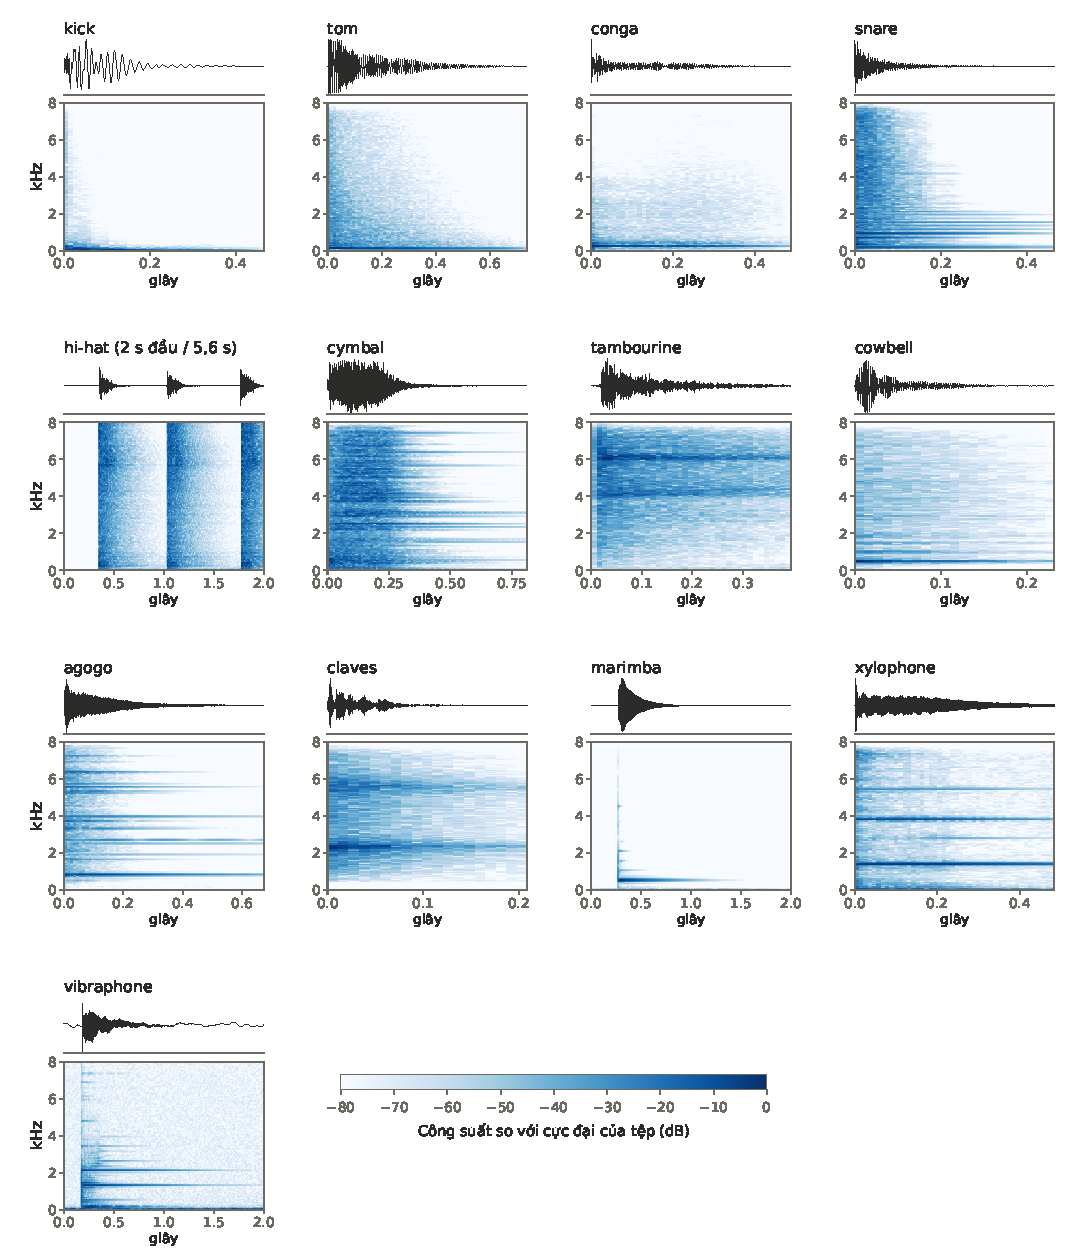
\includegraphics[width=\textwidth]{hinh1_song_va_pho.pdf}
\caption{Dạng sóng (trên) và phổ đồ 0--8 kHz (dưới) của tệp đại diện mỗi nhóm, xếp theo họ nhạc cụ ở Bảng~\ref{tab:phanloai}. Tệp hi-hat lấy từ IDMT, marimba và vibraphone lấy từ Iowa, các tệp còn lại lấy từ Freesound. Mỗi ô có trục thời gian riêng theo độ dài tệp, tối đa 2 s; tệp hi-hat là chuỗi nhiều lần đánh nên chỉ vẽ 2 s đầu. Màu đậm là công suất gần cực đại của tệp. Năng lượng của kick, tom, conga tập trung dưới 0,5 kHz nên chỉ chiếm dải hẹp ở đáy phổ đồ.}\label{fig:pho}
\end{figure}

Các đặc điểm nổi bật trên những tệp minh họa:
\begin{itemize}
\item \textbf{Trống màng rung trầm (kick, tom, conga):} năng lượng dồn vào vài vạch tần số thấp. Trên tệp đại diện, phổ trung bình có đỉnh ở khoảng 52 Hz với kick, 122 Hz với tom, và ở 232 Hz cùng 393 Hz với conga. Ngoài các vạch này chỉ có một vệt dọc rất ngắn lúc vừa gõ, trải trên nhiều tần số. Tom ngân lâu hơn kick và conga.
\item \textbf{Snare:} giống ba trống trên ở các vạch dưới 1,5 kHz do thân trống tạo ra. Điểm khác là trong khoảng 0,2 s đầu có thêm một vùng năng lượng giống nhiễu trải tới 8 kHz, do dây lò xo rung.
\item \textbf{Hi-hat và cymbal:} cả hai đều có năng lượng dày đặc, phủ gần hết dải 0--8 kHz. Hai nhạc cụ khác nhau ở thời gian: cymbal ngân lâu với nhiều vạch đan xen, còn mỗi lần đánh hi-hat chỉ là một vệt dọc ngắn, lặp lại theo nhịp.
\item \textbf{Tambourine:} cũng sáng như hi-hat, nhưng năng lượng không trải đều mà dồn vào hai dải hẹp quanh 4,1--4,8 kHz và 6,1--6,3 kHz, kéo dài suốt tệp.
\item \textbf{Cowbell và agogo:} đều là chuông kim loại với vài vạch tần số rời rạc. Vạch của cowbell nằm thấp (khoảng 0,48 và 1,0 kHz) và tắt nhanh. Vạch của agogo cao hơn (khoảng 0,8; 2,7; 4,0 và 5,6 kHz) và ngân lâu hơn.
\item \textbf{Claves:} rất ngắn (khoảng 0,2 s), năng lượng tập trung ở hai cụm quanh 2,1--2,5 kHz và 5,5--5,8 kHz.
\item \textbf{Marimba, xylophone, vibraphone:} cả ba đều có các vạch nằm ngang rõ nét, vì mỗi thanh gõ được chỉnh để phát ra một nốt nhạc xác định. Marimba gần như chỉ có một vạch chính (khoảng 0,53 kHz, gần nốt C5). Xylophone có các vạch ở 1,4 và 3,8 kHz. Vibraphone có các vạch dưới 2,2 kHz, ngân suốt 2 s.
\end{itemize}

\subsection{Mô tả 13 nhóm và các dấu hiệu so sánh}
Bảng~\ref{tab:mota} tổng hợp đặc điểm và các nhóm dễ nhầm, dựa trên cấu tạo nhạc cụ, phổ đồ và thống kê của tập dữ liệu.
\begin{table}[htbp]
\centering\small
\caption{Đặc điểm của 13 nhóm nhạc cụ và nhóm dễ nhầm lẫn với chúng.}\label{tab:mota}
\begin{tabularx}{\textwidth}{p{.15\textwidth}X}
\toprule
Nhạc cụ & Đặc điểm và điểm so sánh đáng chú ý\\\midrule
Kick & Thân tiếng rất trầm, xung năng lượng mạnh và tắt nhanh. Gần tom và conga ở năng lượng thấp; khác ở vị trí vạch trầm và diễn biến năng lượng.\\
Tom & Cộng hưởng mặt trống, có thân tiếng và đuôi suy giảm dài hơn kick. Gần conga nhất trong bộ dữ liệu.\\
Conga & Trống tay; tiếng thay đổi theo cách đánh mở, hãm hoặc vỗ. Phần trầm gần tom, phần đầu tiếng thay đổi mạnh theo kỹ thuật.\\
Snare & Thân tiếng trống kết hợp phần rè của dây lò xo, nên phổ phân tán hơn các trống trầm và gần cymbal ở thành phần nhiễu.\\
Hi-hat & Tiếng kim loại sáng, phổ gần giống nhiễu; đóng hay mở tạo độ ngân khác nhau. Gần tambourine về độ sáng, gần cymbal và snare về độ phân tán.\\
Cymbal & Nhiều thành phần kim loại, phổ trải rộng, đuôi ngân dài. Có chung tính nhiễu với hi-hat và snare.\\
Tambourine & Các miếng kim loại nhỏ tạo tiếng leng keng ở dải cao, tập trung vào vài dải hẹp. Trọng tâm phổ cao nhất bộ dữ liệu.\\
Cowbell & Chuông kim loại với vài vạch cộng hưởng thấp, tắt nhanh. Cùng kiểu vạch rời rạc với agogo nhưng vạch nằm thấp hơn.\\
Agogo & Chuông gõ với các vạch cộng hưởng rời rạc ở dải trung và cao; cỡ chuông và lực đánh làm dịch vạch. Phân biệt với cowbell nhờ vị trí vạch.\\
Claves & Va chạm hai thanh gỗ, rất ngắn và sắc, năng lượng tập trung ở vài kHz. Khởi âm rõ như nhiều nhạc cụ khác nhưng đuôi tiếng ngắn nhất.\\
Marimba & Thanh gỗ có cao độ, có ống cộng hưởng; năng lượng dồn vào vạch cơ bản, vạch cao tắt nhanh. Cao độ nốt làm dịch toàn bộ phổ.\\
Vibraphone & Thanh kim loại có cao độ, ngân dài nếu không hãm tiếng. Gần marimba về độ tập trung phổ.\\
Xylophone & Thanh gỗ có cao độ, âm sáng và khởi âm rõ. Trong bộ dữ liệu có trọng tâm phổ cao hơn hẳn marimba và vibraphone.\\\bottomrule
\end{tabularx}
\end{table}

\FloatBarrier
\section{So sánh định lượng tiếng nhạc cụ}\label{sec:dinhluong}
\subsection{Cách đọc số liệu}
Bảng~\ref{tab:acoustic} trình bày \textbf{trung vị theo lớp} của các đặc trưng trung bình theo khung hợp lệ 25 ms. Ký hiệu và công thức được dùng thống nhất với Mục~\ref{sec:quytrinh}--\ref{sec:boA-pho}.
\begin{table}[H]
\centering\small
\caption{Trung vị theo lớp của các đại lượng phổ trung bình theo khung. $C$: trọng tâm phổ; $F$: độ phẳng phổ; $H$: entropy phổ; $L$: tỷ lệ năng lượng dưới 500 Hz; $\Phi$: thông lượng phổ.}\label{tab:acoustic}
\begin{tabular}{lrrrrr}
\toprule
Nhãn & $C$ (Hz) & $F$ & $H$ & $L$ (\%) & $\Phi$\\\midrule
agogo & 1.261,3 & 0,0015 & 0,272 & $<0{,}01$ & 0,045 \\
claves & 2.668,7 & 0,0121 & 0,458 & $<0{,}01$ & 0,363 \\
conga & 240,6 & 0,0001 & 0,256 & 99,61 & 0,117 \\
cowbell & 720,6 & 0,0036 & 0,252 & 42,04 & 0,141 \\
cymbal & 2.838,4 & 0,0910 & 0,710 & 3,38 & 0,338 \\
hi-hat & 4.429,7 & 0,2945 & 0,839 & 9,23 & 0,403 \\
kick & 60,3 & 0,0002 & 0,229 & 99,84 & 0,188 \\
marimba & 245,2 & 0,0002 & 0,219 & 78,91 & 0,059 \\
snare & 1.749,6 & 0,1661 & 0,696 & 29,89 & 0,353 \\
tambourine & 5.766,8 & 0,0211 & 0,584 & 0,01 & 0,397 \\
tom & 144,0 & 0,0007 & 0,234 & 99,20 & 0,088 \\
vibraphone & 307,9 & 0,0003 & 0,198 & 76,85 & 0,053 \\
xylophone & 1.889,3 & 0,0003 & 0,254 & 5,85 & 0,070 \\
\bottomrule
\end{tabular}
\end{table}

\begin{figure}[H]
\centering
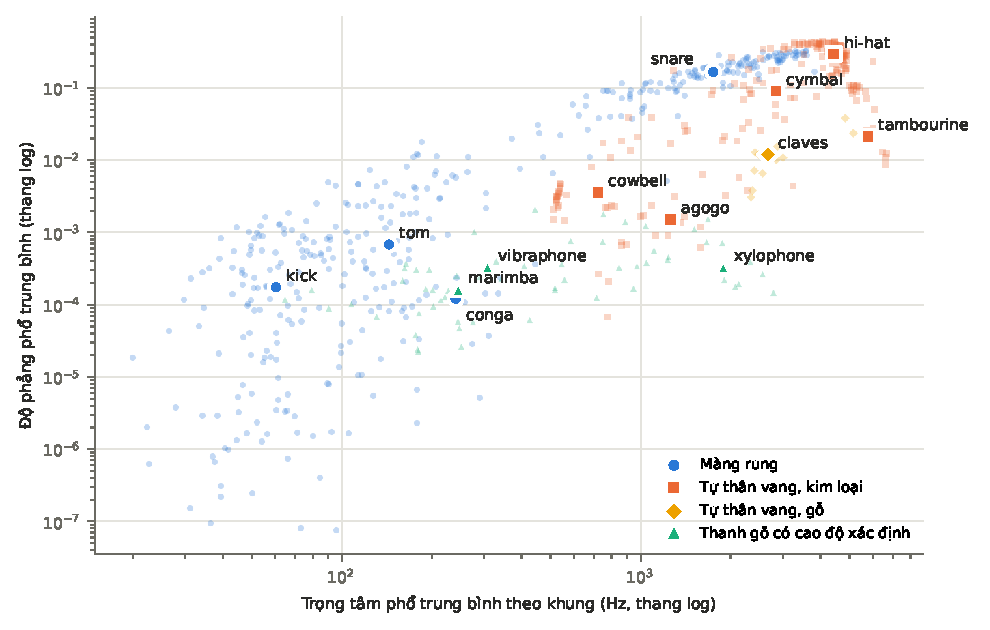
\includegraphics[width=.78\textwidth]{hinh2_trong_tam_do_phang.pdf}
\caption{Trọng tâm phổ và độ phẳng phổ của 655 tệp (điểm nhạt) và trung vị từng lớp (điểm đậm có nhãn), tô màu và phân biệt hình dạng điểm theo bốn họ nhạc cụ ở Bảng~\ref{tab:phanloai}. Cả hai trục dùng thang logarit.}\label{fig:phantan}
\end{figure}

\subsection{Những tương đồng và khác biệt quan sát được}
\textbf{Kick, tom và conga} chồng lấn ở vùng trọng tâm thấp trên Hình~\ref{fig:phantan}.

\textbf{Hi-hat, cymbal và snare} thuộc nhóm phổ phân tán. Tambourine cũng giàu cao tần nhưng năng lượng dồn vào một số dải, nên có độ phẳng thấp hơn nhiều so với hi-hat.

\textbf{Marimba và vibraphone} có entropy thấp nhất tập. Xylophone có trọng tâm cao hơn; so sánh này chịu ảnh hưởng đồng thời của âm vực và nguồn mẫu khác nhau (Freesound so với Iowa).

\textbf{Agogo và cowbell} khác nhau rõ ở dải thấp: $L$ lần lượt khoảng 0,002\% và 42,04\%, với các vạch cộng hưởng của cowbell nằm thấp hơn.
\clearpage

\phan{Các bộ đặc trưng nhận diện âm thanh}
\section{Quy trình biểu diễn âm thanh}\label{sec:quytrinh}
\subsection{Từ tệp âm thanh đến vector đặc trưng}
Mỗi tệp được biểu diễn bằng vector có số chiều cố định. Quy trình trích đặc trưng và so sánh gồm tám bước:
\begin{enumerate}
\item đọc tệp WAV;
\item bỏ thành phần một chiều (DC) và chuẩn hóa đỉnh, để mọi tệp có cùng biên độ lớn nhất;
\item xác định vùng có tiếng (vùng có tín hiệu);
\item chia tín hiệu thành các khung ngắn;
\item tính các đại lượng thời gian, phổ và MFCC;
\item tổng hợp các giá trị theo khung thành giá trị của cả tệp;
\item chuẩn hóa các thuộc tính về cùng một thang đo;
\item tính khoảng cách giữa hai vector.
\end{enumerate}
Các bước 1--6 được thực hiện khi đưa tệp vào kho; bước 7--8 dùng để chuẩn hóa và so sánh với truy vấn.

Với tín hiệu đầu vào $x[n]$ có $N$ mẫu, bước loại DC và chuẩn hóa đỉnh được thực hiện theo
\[
y[n]=\frac{x[n]-\bar{x}}{\max_n|x[n]-\bar{x}|},\qquad
\bar{x}=\frac{1}{N}\sum_{n=0}^{N-1}x[n].
\]
Tín hiệu $y[n]$ có trung bình bằng 0 và biên độ đỉnh bằng 1. Cách xử lý này loại ảnh hưởng của thay đổi hệ số khuếch đại tuyến tính; độ to tuyệt đối không được dùng làm thuộc tính.

\begin{table}[htbp]
\centering\small
\caption{Thiết lập xử lý tín hiệu dùng cho cả ba bộ đặc trưng.}\label{tab:thietlap}
\begin{tabularx}{\textwidth}{p{.31\textwidth}X}
\toprule
Thành phần & Thiết lập đã dùng\\\midrule
Tín hiệu đầu vào & Mono, $f_s=16.000$ Hz; tính toán bằng số thực 64-bit.\\
Bao RMS cho thời gian & Các khối 160 mẫu (10 ms), không chồng nhau; khối cuối có thể ngắn hơn. Khối có tín hiệu khi RMS $>0{,}01$ sau chuẩn hóa đỉnh.\\
Khung phân tích phổ & 400 mẫu (25 ms), bước 160 mẫu (10 ms), bắt đầu từ mẫu đầu tiên của tệp. Số khung là $\max\big(1,\lceil(N-400)/160\rceil+1\big)$; khung cuối được thêm số 0 cho đủ 400 mẫu.\\
Khung phổ hợp lệ & RMS trước khi nhân cửa sổ $>0{,}01$; cửa sổ Hann dạng tuần hoàn. Nếu không có khung nào hợp lệ, dùng khung có năng lượng lớn nhất.\\
Biến đổi phổ & FFT 512 điểm; 257 bin từ 0 đến 8 kHz, bước bin 31,25 Hz.\\
Tổng hợp & Trung bình và độ lệch chuẩn tổng thể (chia cho số khung hợp lệ) trên các khung hợp lệ; thông lượng phổ và delta có điều kiện hợp lệ riêng.\\\bottomrule
\end{tabularx}
\end{table}
Phổ công suất của khung $t$ là $P_t[k]=|\mathrm{FFT}(y_t w)[k]|^2$, với $f_k=16000k/512$, $k=0,\ldots,256$ và cửa sổ Hann $w$. Phổ được chuẩn hóa theo tổng công suất của từng khung:
\[
q_t[k]=\frac{P_t[k]}{\sum_{j=0}^{256}P_t[j]},
\]
Mẫu số được chặn dưới ở $10^{-30}$. Các đại lượng phổ dùng $q_t$, riêng thông lượng phổ dùng $\sqrt{q_t}$. FFT 512 điểm trên khung 400 mẫu tạo bước bin 31,25 Hz; phần thêm số 0 không tăng độ phân giải thực của phép phân tích.

\subsection{Ba bộ đặc trưng được xây dựng}
\begin{itemize}
\item \textbf{Bộ A (21 chiều):} 5 thuộc tính thời gian và 16 thuộc tính tổng hợp theo khung, mô tả thời lượng hoạt động, bao âm và phân bố phổ (Mục~\ref{sec:boA-tg}--\ref{sec:boA-pho}).
\item \textbf{Bộ B (39 chiều):} các thống kê của hệ số MFCC, mô tả hình dạng tổng thể của phổ và mức thay đổi của nó theo thời gian (Mục~\ref{sec:boB}).
\item \textbf{Bộ C (60 chiều):} ghép A và B sau khi chuẩn hóa, có trọng số để hai phần đóng góp ngang nhau (Mục~\ref{sec:boC}).
\end{itemize}
Mọi thuộc tính đều được tính từ chính âm thanh. Nhãn nhạc cụ không nằm trong vector, mà chỉ dùng để đánh giá kết quả.

\subsection{Đối chiếu với các nhóm đặc trưng âm thanh thông dụng}
Theo cách phân nhóm trong tài liệu về đặc trưng âm thanh~\cite{peeters}, các thuộc tính đã chọn thuộc hai miền:
\begin{itemize}
\item \textbf{Miền thời gian:} thời gian hoạt động $a_1$, khoảng chứa 90\% năng lượng $a_2$, hệ số đỉnh $a_3$, tỷ lệ có tín hiệu $a_4$, vị trí đỉnh bao RMS $a_5$ và tỷ lệ đổi dấu ZCR. Trong tổ chức vector, ZCR được ghép với các đại lượng phổ vì cùng tính trên khung 25 ms.
\item \textbf{Miền tần số:} trọng tâm $C$, tần số cắt $R$, tỷ lệ năng lượng thấp $L$, độ rộng $W$, độ phẳng $F$, entropy $H$, thông lượng phổ và MFCC.
\end{itemize}
Cao độ và độ hài hòa chưa được đưa vào bộ đặc trưng. Phần lớn lớp có phổ phi hài hòa hoặc không có cao độ xác định; với ba lớp thanh gõ, tần số cơ bản còn phụ thuộc nốt được chơi. Độ phẳng và entropy được dùng để mô tả mức tập trung phổ.

\section{Bộ A: năm thuộc tính thời gian}\label{sec:boA-tg}
Năm thuộc tính thời gian được tính từ các khối 10 ms (160 mẫu), không chồng nhau. Khối có RMS sau chuẩn hóa đỉnh lớn hơn 0,01 được coi là \emph{có tín hiệu}. Các ký hiệu gồm:
\begin{itemize}
\item $\mathcal A$: tập các mẫu thuộc những khối có tín hiệu;
\item $n_0, n_1$: vị trí của mẫu có tín hiệu đầu tiên và cuối cùng;
\item $T_a=|\mathcal A|/f_s$: tổng thời gian có tín hiệu, tính bằng giây;
\item $T_s=(n_1-n_0+1)/f_s$: khoảng thời gian từ lúc vùng có tín hiệu bắt đầu đến lúc kết thúc, kể cả các khoảng nghỉ ở giữa.
\end{itemize}
Ví dụ, một tệp có hai tiếng gõ, mỗi tiếng dài 0,2 s và cách nhau 0,5 s im lặng, sẽ có $T_a\approx0{,}4$ s và $T_s\approx0{,}9$ s.

\subsection{Thời gian có tín hiệu và khoảng chứa 90\% năng lượng}
\[
a_1=\ln(1+T_a),\qquad a_2=\ln(1+D_{90}),\qquad
D_{90}=\frac{n_{95}-n_{05}}{f_s},
\]
trong đó $n_p$ là vị trí mẫu đầu tiên mà năng lượng cộng dồn đạt $p\%$ tổng năng lượng $\sum_n y[n]^2$. Phép $\ln(1+\cdot)$ nén khoảng thời lượng từ 0,1 s đến hơn 20 s của tập dữ liệu.

$T_a$ đo tổng thời gian hoạt động, còn $D_{90}$ phản ánh mức tập trung năng lượng theo thời gian. Tiếng claves ngắn thường có $D_{90}$ nhỏ; tiếng cymbal ngân hoặc chuỗi nhiều lần đánh có thể trải năng lượng trên khoảng dài hơn. Với chuỗi, khoảng đo bao gồm cả những lần đánh và khoảng nghỉ nằm giữa hai mốc năng lượng.

\Needspace{8\baselineskip}
\subsection{Hệ số đỉnh trên vùng có tín hiệu}
\[
a_3=20\log_{10}\left(\frac{1}{\sqrt{|\mathcal A|^{-1}\sum_{n\in\mathcal A}y[n]^2}}\right)\quad\text{(dB)}.
\]
Hệ số đỉnh (crest factor) đo chênh lệch giữa biên độ đỉnh và RMS trên vùng có tín hiệu. Giá trị lớn ứng với xung nổi bật trên nền năng lượng thấp; giá trị nhỏ ứng với biên độ duy trì đều hơn. Nén dải động, cách chơi và số lần đánh trong tệp đều ảnh hưởng đến thuộc tính này.

\subsection{Tỷ lệ có tín hiệu và vị trí đỉnh bao RMS}
\[
a_4=\frac{T_a}{T_s},\qquad
 a_5=\min\left(\max\left(\frac{160b_{\max}-n_0}{\max(n_1-n_0,1)},\,0\right),\,1\right),
\]
trong đó $b_{\max}$ là chỉ số khối 10 ms có RMS lớn nhất; $a_5$ được chặn trong $[0,1]$.

$a_4$ giảm khi bản ghi có nhiều khoảng nghỉ. Với ví dụ hai tiếng gõ ở đầu mục, $a_4\approx0{,}4/0{,}9\approx0{,}44$. Vị trí $a_5$ gần 0 ứng với đỉnh bao RMS ở đầu vùng hoạt động, còn giá trị lớn hơn ứng với đỉnh đến muộn. Trong chuỗi nhiều lần đánh, thuộc tính này chỉ ghi vị trí khối mạnh nhất của cả chuỗi.

\section{Bộ A: tám đại lượng phổ và cách tổng hợp}\label{sec:boA-pho}
Các đại lượng phổ được tính trên khung hợp lệ theo Bảng~\ref{tab:thietlap}, rồi tổng hợp bằng trung bình và độ lệch chuẩn.
\subsection{Vị trí và độ trải rộng năng lượng}
\textbf{Trọng tâm phổ} (spectral centroid) và \textbf{độ rộng phổ} (bandwidth) được tính theo
\[
C_t=\sum_k f_kq_t[k],\qquad W_t=\sqrt{\sum_k(f_k-C_t)^2q_t[k]}.
\]
$C_t$ và $W_t$ có đơn vị Hz, lần lượt mô tả vị trí trung bình và độ trải của năng lượng theo tần số. $C_t$ phản ánh độ sáng phổ, còn cao độ của nốt gắn với tần số cơ bản.

\textbf{Tần số cắt 85\%} (rolloff) là $R_t=f_{k^*}$ với $k^*=\min\{k:\sum_{j=0}^kq_t[j]\geq0{,}85\}$. Thuộc tính này xác định mốc tần số chứa ít nhất 85\% năng lượng của khung ở phía dưới hoặc tại mốc đó.

\textbf{Tỷ lệ năng lượng thấp} $L_t=\sum_{f_k<500\,\mathrm{Hz}}q_t[k]$ đo phần năng lượng dưới 500 Hz trong từng khung. Giá trị của tệp là trung bình trên các khung hợp lệ, mỗi khung có trọng số ngang nhau. Các khung đuôi yếu còn vượt ngưỡng RMS vẫn được tính như khung mạnh; vì thế kết quả khác với tỷ lệ tính từ phổ công suất cộng gộp của cả tệp.

\subsection{Độ tập trung và tính nhiễu của phổ}
\textbf{Độ phẳng phổ} (spectral flatness) là tỷ số giữa trung bình nhân và trung bình cộng của công suất trên 257 bin:
\[
F_t=\frac{\exp\left(\frac{1}{K}\sum_k\ln\widetilde P_t[k]\right)}{\frac{1}{K}\sum_k\widetilde P_t[k]},\qquad K=257,
\]
trong đó $\widetilde P_t[k]=\max(P_t[k],10^{-12}\max(\max_jP_t[j],10^{-30}))$ bảo đảm đối số logarit dương. $F_t$ gần 0 với phổ tập trung vào vài vạch và bằng 1 với phổ công suất đều trên mọi bin.

\textbf{Entropy phổ chuẩn hóa} $H_t=-\sum_kq_t[k]\ln q_t[k]/\ln K$ (quy ước $0\ln0=0$) nằm trong $[0,1]$ và tăng theo mức phân tán năng lượng. Entropy và độ phẳng có phản ứng khác nhau với các bin công suất nhỏ, nên cả hai được giữ trong bộ A.

\subsection{Mức dao động và thay đổi giữa các khung}
\textbf{Tỷ lệ đổi dấu (ZCR):} $Z_t=\frac{1}{399}\sum_{n=1}^{399}\mathbf1\big[(y_t[n]<0)\ne(y_t[n-1]<0)\big]$ được tính trên khung trước khi nhân cửa sổ. ZCR thường cao ở các tiếng giàu cao tần hoặc có tính nhiễu.

\textbf{Thông lượng phổ dương} (spectral flux) $\Phi_t=\sqrt{\sum_k[\max(\sqrt{q_t[k]}-\sqrt{q_{t-1}[k]},0)]^2}$ đo phần tăng của phổ chuẩn hóa giữa hai khung liền nhau. Giá trị lớn thường xuất hiện ở khởi âm hoặc khi phổ đổi nhanh. Chỉ các cặp khung đều hợp lệ mới được tính; tệp không có cặp hợp lệ nhận giá trị thông lượng bằng 0.

\subsection{Từ tám chuỗi giá trị thành 16 thuộc tính}\label{sec:tonghop}
Trên $M$ khung hợp lệ, mỗi chuỗi $v_t$ được tổng hợp thành trung bình $\mu_v$ và độ lệch chuẩn tổng thể $\sigma_v=\sqrt{M^{-1}\sum_t(v_t-\mu_v)^2}$. Tám cặp thống kê tạo thành 16 thuộc tính, ghép với 5 thuộc tính thời gian để có \textbf{bộ A gồm 21 chiều}. Báo cáo gọi tắt nhóm 16 thuộc tính là \emph{khối phổ}, gồm cả ZCR tính trên dạng sóng.

\section{Bộ B: MFCC và thông tin về bao phổ}\label{sec:boB}
\subsection{Từ phổ công suất đến hệ số cepstrum}
Bộ B dùng 13 hệ số MFCC (Mel-frequency cepstral coefficients)~\cite{mfcc} để biểu diễn bao phổ. Quy trình gồm lọc theo thang Mel, lấy logarit năng lượng dải và biến đổi cosine rời rạc (DCT).

\textbf{Bước 1, chia dải theo thang Mel.} Dùng 40 bộ lọc tam giác trong dải 20 Hz--8 kHz, với các điểm biên cách đều trên thang Mel kiểu HTK:
\[
m(f)=2595\log_{10}(1+f/700).
\]
42 điểm biên tạo ra 40 tam giác. Trọng số $H_b[k]$ của mỗi bộ lọc được chuẩn hóa sao cho tổng trên 257 bin bằng 1.

\textbf{Bước 2, lấy logarit năng lượng từng dải.} Năng lượng và logarit năng lượng của dải $b$ là
\[
E_t[b]=\sum_k H_b[k]P_t[k],\qquad \ell_t[b]=\ln\max(E_t[b],10^{-10}),\quad b=0,\ldots,39.
\]
Năng lượng dải được chặn dưới ở $10^{-10}$ trước khi lấy logarit.

\textbf{Bước 3, DCT.} Áp dụng DCT loại II chuẩn trực giao lên 40 giá trị logarit và giữ các hệ số $r=1,\ldots,13$:
\[
c_t[r]=\sqrt{\frac{2}{40}}\sum_{b=0}^{39}\ell_t[b]\cos\left[\frac{\pi r}{40}\left(b+\frac12\right)\right].
\]
Các hệ số bậc thấp mô tả xu hướng tổng thể của bao phổ, các bậc sau giữ chi tiết hơn. Hệ số $c_0$ bị loại để giảm ảnh hưởng của mức năng lượng chung. DCT được tính bằng SciPy~\cite{dct}; cấu hình lọc, logarit và chọn hệ số được dùng thống nhất cho kho dữ liệu và truy vấn.

\subsection{Ba nhóm thống kê, tổng cộng 39 chiều}
Mỗi chuỗi hệ số MFCC được tổng hợp thành:
\begin{itemize}
\item \textbf{trung bình} của 13 hệ số trên các khung hợp lệ: 13 giá trị;
\item \textbf{độ lệch chuẩn} của 13 hệ số: 13 giá trị;
\item \textbf{độ lệch chuẩn của delta}: 13 giá trị.
\end{itemize}
Delta là tốc độ thay đổi của mỗi hệ số theo thời gian, tính trên năm khung liên tiếp:
\[
\Delta c_t[r]=\frac{c_{t+1}[r]-c_{t-1}[r]+2(c_{t+2}[r]-c_{t-2}[r])}{10}.
\]
Ở hai đầu chuỗi, giá trị đầu và cuối được lặp lại để đủ năm khung. Một giá trị delta chỉ được dùng khi cả năm khung đều hợp lệ; nếu tệp không có giá trị delta nào dùng được thì độ lệch chuẩn delta được gán bằng 0. Tổng cộng, bộ B có \textbf{39 chiều} ($13+13+13$).

\subsection{Giá trị thông tin và giới hạn}
Trung bình MFCC giữ hình dạng bao phổ điển hình, độ lệch chuẩn ghi mức biến thiên trong tệp, còn thống kê delta nhấn mạnh biến đổi cục bộ như ở khởi âm. Cách biểu diễn này có thể phân biệt các âm có trọng tâm gần nhau nhưng phân bố năng lượng giữa các dải khác nhau.

MFCC nhạy với nốt được chơi, cách thu và xử lý cân bằng phổ (EQ). Việc tổng hợp bằng trung bình và độ lệch chuẩn cũng làm mất thứ tự các sự kiện. Ảnh hưởng của biến thiên trong lớp được xét cụ thể với marimba và vibraphone ở Mục~\ref{sec:cap}.

\section{Bộ C và phép đo tương đồng}\label{sec:boC}
\subsection{Chuẩn hóa để so sánh các thuộc tính khác đơn vị}\label{sec:chuanhoa}
Trước khi tính khoảng cách, các thuộc tính được chuẩn hóa theo độ lệch chuẩn để giảm ảnh hưởng của khác biệt đơn vị và thang giá trị:
\[
z_j(x)=\frac{x_j-\mu_j}{s_j},
\]
trong đó $\mu_j$ và $s_j$ được tính trên 655 tệp; $s_j<10^{-12}$ được thay bằng 1. Các tham số này được lưu cùng kho và dùng lại khi chuẩn hóa truy vấn.

Gọi $z_A\in\mathbb R^{21}$ và $z_B\in\mathbb R^{39}$ là hai vector đã chuẩn hóa. Vector dùng để tính khoảng cách của từng bộ là
\[
u_A=\frac{z_A}{\sqrt{21}},\qquad
u_B=\frac{z_B}{\sqrt{39}},\qquad
u_C=\left[\frac{z_A}{\sqrt{42}},\frac{z_B}{\sqrt{78}}\right].
\]
Hệ số chia theo số chiều cân bằng quy mô khoảng cách giữa hai bộ. Trong vector C gồm \textbf{60 chiều}, mỗi phần A và B có trọng số $1/2$ trong bình phương khoảng cách.

\subsection{Khoảng cách biểu diễn cả giống và khác nhau}
Khoảng cách giữa hai tệp được tính bằng chuẩn Euclid:
\[
d_S(x,y)=\|u_S(x)-u_S(y)\|_2,\qquad S\in\{A,B,C\}.
\]
Các tệp được xếp theo khoảng cách tăng dần; những chiều có chênh lệch lớn được dùng để giải thích khác biệt. Với bộ C,
\[
\boxed{d_C^2(x,y)=\tfrac12d_A^2(x,y)+\tfrac12d_B^2(x,y).}
\]
Đẳng thức áp dụng cho bình phương khoảng cách của từng cặp tệp. Các khoảng cách trung bình ở Mục~\ref{sec:sodo} được tính trực tiếp từ từng biểu diễn. Điểm hiển thị $s=1/(1+d)$ bảo toàn thứ tự tương đồng và mang ý nghĩa thang điểm, không mang ý nghĩa xác suất cùng nhãn.

\subsection{Sử dụng khi lưu trữ và tìm kiếm}\label{sec:sudung}
\textbf{Dữ liệu cần lưu.} Với mỗi tệp, cơ sở dữ liệu lưu mã tệp, nhãn, đường dẫn, thông tin nguồn và giá trị gốc (chưa chuẩn hóa) của 21 thuộc tính bộ A và 39 thuộc tính bộ B, theo đúng thứ tự ở Phụ lục. Ngoài ra, cả kho chỉ cần lưu một lần 60 cặp tham số chuẩn hóa $\mu_j, s_j$. Các vector $u_A$, $u_B$, $u_C$ tính được từ những giá trị này theo Mục~\ref{sec:chuanhoa}, nên có thể lưu sẵn để tìm nhanh hơn hoặc tính lại khi cần.

\textbf{Xử lý âm thanh truy vấn.} Tệp truy vấn có thể có định dạng, số kênh hay tần số lấy mẫu bất kỳ, nên trước hết phải được đưa về đúng dạng của kho: một kênh, 16 kHz. Sau đó, tệp đi qua đúng các bước 1--6 ở Mục~\ref{sec:quytrinh} với thiết lập ở Bảng~\ref{tab:thietlap}, rồi được chuẩn hóa bằng $\mu_j, s_j$ đã lưu. Một số trường hợp đặc biệt cần xử lý:
\begin{itemize}
\item tệp im lặng hoàn toàn, hoặc không có khối 10 ms nào có RMS lớn hơn 0,01, thì không tính được đặc trưng và cần bị từ chối;
\item nếu không có khung phổ nào hợp lệ, dùng khung có năng lượng lớn nhất thay thế;
\item nếu không có cặp khung liền nhau hợp lệ, thông lượng phổ bằng 0; nếu không có giá trị delta nào dùng được, độ lệch chuẩn delta bằng 0.
\end{itemize}
Các điều kiện chất lượng ở Mục~\ref{sec:curation} cũng được áp dụng cho truy vấn.

\textbf{Tìm 5 tệp giống nhất.} Tính $d_S$ từ truy vấn đến các tệp trong kho, sắp xếp tăng dần và lấy 5 kết quả đầu. Truy vấn trùng một tệp trong kho sẽ loại chính tệp đó khỏi kết quả. Nhóm đề xuất A làm bộ mặc định ban đầu vì dễ diễn giải và có $Q$ cao nhất trong ba bộ A, B, C; lựa chọn cuối cùng dựa trên đánh giá tìm kiếm ở Yêu cầu 4 (Mục~\ref{sec:chonbo}).

\textbf{Nhạc cụ ngoài 13 lớp.} Hệ thống trả về các tệp gần nhất theo đặc trưng âm thanh, dù kho chưa có nhãn tương ứng với nhạc cụ truy vấn.

\section{Giá trị thông tin thể hiện qua số liệu}\label{sec:sodo}
\subsection{So sánh khoảng cách trong lớp và giữa các lớp}
Gọi $\mathcal D_c$ là tập tệp có nhãn $c$, $n_c=|\mathcal D_c|$ và $G=13$. Khoảng cách trung bình trong lớp được tính đều trên 13 lớp:
\[
D_{\rm trong}=\frac1G\sum_c\frac{2}{n_c(n_c-1)}\sum_{i<j;\ i,j\in\mathcal D_c}d(i,j).
\]
Khoảng cách trung bình giữa lớp được tính đều trên $\binom{13}{2}=78$ cặp lớp:
\[
D_{\rm ngoài}=\frac{1}{\binom G2}\sum_{c<d}\frac{1}{n_cn_d}\sum_{i\in\mathcal D_c}\sum_{j\in\mathcal D_d}d(i,j).
\]
Tỷ số $Q=D_{\rm ngoài}/D_{\rm trong}$ được dùng để so sánh mức tách lớp của các biểu diễn. Cách lấy trung bình trên lớp và cặp lớp giảm ảnh hưởng của chênh lệch số mẫu giữa kick, snare và các lớp nhỏ.
\begin{table}[H]
\centering
\caption{Khoảng cách trong lớp, giữa lớp và tỷ số $Q$ trên toàn bộ 655 tệp.}\label{tab:Q}
\begin{tabular}{lrrrr}
\toprule
Bộ & Số chiều & $D_{\rm trong}$ & $D_{\rm ngoài}$ & $Q$\\\midrule
A & 21 & 0,731 & 1,269 & 1,735 \\
B & 39 & 1,168 & 1,607 & 1,376 \\
C & 60 & 1,010 & 1,487 & 1,473 \\
\bottomrule
\end{tabular}
\end{table}
Trong ba bộ, \textbf{A đạt $Q$ cao nhất (1,735)}, tiếp đến C (1,473) và B (1,376). Ghép MFCC vào A làm giảm tỷ số này trên tập hiện tại. $Q$ phản ánh khoảng cách trung bình toàn cục; chất lượng top-5 cần được đánh giá riêng, cả trên mọi truy vấn và theo trung bình đều giữa các lớp.

\Needspace{7\baselineskip}
\subsection{Kiểm tra ảnh hưởng của chuỗi dài lên tỷ số \texorpdfstring{$Q$}{Q}}
Nhóm tính lại $Q$ cho riêng hai khối thuộc tính của A và trên tập con 563 tệp dài không quá 2 s. Tập con được chuẩn hóa lại bằng các tham số tính từ chính tập đó. Kết quả ở Bảng~\ref{tab:Qtach} giữ thứ tự A $>$ C $>$ B sau khi loại 92 chuỗi IDMT dài.
\begin{table}[H]
\centering
\caption{Tỷ số $Q$ theo khối thuộc tính và theo tập tệp.}\label{tab:Qtach}
\begin{tabular}{lrrr}
\toprule
Biểu diễn & Số chiều & $Q$ (655 tệp) & $Q$ (563 tệp $\le$ 2 s)\\\midrule
A, chỉ 5 thuộc tính thời gian & 5 & 1,350 & 1,515 \\
A, chỉ 16 thuộc tính phổ & 16 & 1,927 & 1,979 \\
A & 21 & 1,735 & 1,782 \\
B & 39 & 1,376 & 1,368 \\
C & 60 & 1,473 & 1,505 \\
\bottomrule
\end{tabular}
\end{table}
Khối phổ đạt $Q=1{,}927$, cao hơn A đầy đủ (1,735); khối thời gian đạt 1,350. Nhóm giữ năm thuộc tính thời gian để mô tả cấu trúc bản ghi, thay vì tối ưu riêng tỷ số $Q$.

Ảnh hưởng của dạng bản ghi thể hiện rõ ở hi-hat. Khoảng cách trung bình trong 40 tệp ngắn là 0,479, trong 53 chuỗi dài là 0,985, còn giữa hai nhóm là 1,481. Các tệp ngắn và chuỗi dài có xu hướng nằm ở những vùng khác nhau của không gian A, ảnh hưởng đến thứ tự kết quả khi truy vấn bằng một tiếng hi-hat đơn.

\subsection{Ví dụ các cặp nhạc cụ}\label{sec:cap}
Bảng~\ref{tab:cap} dùng hai phép đo: trung bình khoảng cách mọi cặp tệp giữa hai lớp (TB) và khoảng cách giữa hai tâm lớp $\|\bar u_c-\bar u_d\|_2$ (Tâm). Độ phân tán bên trong lớp ảnh hưởng đến TB, còn khoảng cách tâm chỉ xét vị trí trung bình.
\begin{table}[H]
\centering\small
\caption{Khoảng cách giữa một số cặp lớp: trung bình cặp tệp (TB) và khoảng cách tâm lớp (Tâm).}\label{tab:cap}
\begin{tabular}{lrrrrrr}
\toprule
& \multicolumn{2}{c}{Bộ A} & \multicolumn{2}{c}{Bộ B} & \multicolumn{2}{c}{Bộ C}\\
\cmidrule(lr){2-3}\cmidrule(lr){4-5}\cmidrule(lr){6-7}
Cặp nhạc cụ & TB & Tâm & TB & Tâm & TB & Tâm\\\midrule
conga / tom & 0,487 & 0,142 & 0,952 & 0,391 & 0,769 & 0,294 \\
kick / tom & 0,789 & 0,461 & 1,062 & 0,566 & 0,974 & 0,516 \\
snare / cymbal & 0,996 & 0,450 & 0,941 & 0,417 & 0,986 & 0,434 \\
hi-hat / tambourine & 1,307 & 1,093 & 0,838 & 0,413 & 1,130 & 0,826 \\
agogo / cowbell & 0,923 & 0,635 & 2,013 & 1,396 & 1,586 & 1,084 \\
marimba / vibraphone & 0,923 & 0,304 & 2,148 & 0,836 & 1,661 & 0,629 \\
kick / tambourine & 1,642 & 1,508 & 1,188 & 0,780 & 1,450 & 1,200 \\
\bottomrule
\end{tabular}
\end{table}
Trong A, conga/tom có khoảng cách tâm 0,142, còn kick/tambourine đạt 1,508. Cặp hi-hat/tambourine thay đổi đáng kể theo biểu diễn: khoảng cách tâm giảm từ 1,093 ở A xuống 0,413 ở B. MFCC đặt hai lớp giàu cao tần này gần nhau hơn so với các thuộc tính của A.

Với marimba/vibraphone trong B, TB đạt 2,148 trong khi khoảng cách tâm là 0,836. Hai lớp có khoảng cách trong lớp lần lượt 1,964 và 2,097, cao nhất trong 13 lớp; biến thiên MFCC theo nốt được chơi có thể góp phần vào độ phân tán này. Marimba vẫn là lớp có tâm gần vibraphone nhất trong B.

\section{Đóng góp của từng thuộc tính}\label{sec:dongop}
\subsection{Chỉ số phân biệt của từng thuộc tính}
Với trung bình $\mu_{cj}$ và phương sai $\sigma^2_{cj}$ của thuộc tính $j$ trong lớp $c$, chỉ số phân biệt là
\[
J_j=\frac{\operatorname{Var}_{c}(\mu_{cj})}{\frac1{13}\sum_c\sigma^2_{cj}},
\]
$J_j$ so sánh phương sai giữa các trung bình lớp với phương sai trung bình trong lớp. Các phương sai được tính theo tổng thể, mỗi lớp có trọng số bằng nhau; mẫu số được chặn dưới ở $10^{-12}$. Chỉ số này dùng để xếp hạng mô tả các thuộc tính.
\begin{table}[H]
\centering\small
\caption{Chín thuộc tính có $J_j$ cao nhất trong 60 thuộc tính gốc của A và B.}\label{tab:J}
\begin{tabular}{lcr}
\toprule
Thuộc tính & Bộ & $J_j$\\\midrule
MFCC 1, trung bình & B & 8,062 \\
ZCR, trung bình & A & 7,487 \\
Entropy phổ, trung bình & A & 7,145 \\
Trọng tâm phổ, trung bình & A & 7,107 \\
Tần số cắt 85\%, trung bình & A & 6,709 \\
Thông lượng phổ, trung bình & A & 5,921 \\
Độ rộng phổ, trung bình & A & 4,591 \\
Tỷ lệ năng lượng thấp, trung bình & A & 4,217 \\
Độ phẳng phổ, trung bình & A & 3,900 \\
\bottomrule
\end{tabular}
\end{table}
Chín thuộc tính đứng đầu gồm tám thuộc tính của khối phổ A và trung bình MFCC 1. Các thuộc tính thời gian $a_1$--$a_5$ nằm ngoài nhóm này. ZCR, trọng tâm và tần số cắt có phần thông tin trùng nhau do cùng nhạy với thành phần cao tần; xếp hạng riêng lẻ chưa phản ánh tương tác giữa các thuộc tính hoặc khả năng phân biệt từng cặp lớp.

\subsection{Liên hệ với mục tiêu tìm tương đồng và khác biệt}
Bảng~\ref{tab:vaitro} hệ thống hóa vai trò của các nhóm thuộc tính trong tìm kiếm.
\begin{table}[htbp]
\centering\small
\caption{Vai trò của từng nhóm thuộc tính trong việc tìm âm tương đồng và tìm khác biệt.}\label{tab:vaitro}
\begin{tabularx}{\textwidth}{p{.24\textwidth}XX}
\toprule
Nhóm thuộc tính & Dùng để tìm tương đồng & Dùng để tìm khác biệt\\\midrule
Thời gian, hệ số đỉnh & Các tệp có cùng kiểu tập trung năng lượng, tính liên tục và bao âm. & Xung ngắn so với năng lượng kéo dài; đỉnh nhọn so với nền duy trì.\\
Trọng tâm, tần số cắt, $L$ & Cùng giàu âm trầm hoặc cùng sáng. & Trống trầm so với các tiếng kim loại giàu tần số cao.\\
Độ rộng, độ phẳng, entropy phổ & Cùng phổ tập trung hoặc cùng phổ phân tán. & Cộng hưởng nổi bật so với phổ trải rộng; âm sáng có vạch so với âm sáng giống nhiễu.\\
ZCR, thông lượng phổ, các độ lệch chuẩn & Cùng mức dao động và biến đổi giữa các khung. & Phổ ổn định so với phổ đổi nhanh theo kích thích.\\
MFCC và delta & Cùng hình dạng bao phổ và mức biến thiên. & Phân bố năng lượng khác nhau dù trọng tâm hoặc năng lượng thấp tương tự.\\\bottomrule
\end{tabularx}
\end{table}
\clearpage

\section{Tổng kết về dữ liệu và đặc trưng}\label{sec:tongket12}
\subsection{Kết quả cho hai yêu cầu đầu}
Nhóm đã xây dựng bộ dữ liệu 655 tệp thuộc 13 lớp nhạc cụ từ Freesound, IDMT-SMT-Drums và Iowa MIS. Bộ dữ liệu kèm danh mục nguồn, hồ sơ kiểm tra và các bảng đặc trưng, đủ để triển khai phần lưu trữ và truy vấn của đề tài.

Kết quả khảo sát phân biệt rõ nhóm trống trầm với nhóm giàu cao tần. Độ phẳng và entropy bổ sung khác biệt giữa các lớp cùng sáng như hi-hat và tambourine. Riêng các lớp thanh gõ chịu ảnh hưởng đáng kể của nốt được chơi và nguồn thu.

Trong ba biểu diễn đã xây dựng, A đạt tỷ số tách lớp cao nhất. Kết quả tách khối xác định phần đóng góp chính thuộc về các thuộc tính phổ. Chất lượng tìm kiếm top-5 và khả năng áp dụng cho bản thu mới là cơ sở lựa chọn biểu diễn, được đánh giá ở Mục~\ref{sec:danhgia}.

Các tham số chuẩn hóa và chương trình trích đặc trưng được lưu để dùng thống nhất khi xây dựng cơ sở dữ liệu và xử lý truy vấn.

\subsection{Kiểm tra tính toán}
Nhóm đã kiểm tra kết quả tính toán như sau:
\begin{itemize}
\item mọi vector A, B, C đều đủ số chiều và không chứa giá trị lỗi; mã băm của các tệp đầu vào khớp với hồ sơ kiểm kê;
\item không có tệp nào chỉ có một khung phổ hợp lệ hoặc không có giá trị delta nào dùng được, nên hai trường hợp dùng khung thay thế và gán độ lệch chuẩn delta bằng 0 ở Mục~\ref{sec:sudung} không xảy ra với 655 tệp;
\item đặc trưng không đổi khi tăng hay giảm âm lượng của cùng một tín hiệu; phép thử âm sin trầm và nhiễu trắng cho kết quả tỷ lệ năng lượng thấp lớn hơn và độ phẳng nhỏ hơn ở tín hiệu sin.
\end{itemize}

Đặc trưng được tính bằng các thư viện NumPy 2.4.6, SciPy 1.17.1 và SoundFile 0.13.1; các số trong bảng đã được làm tròn. Nhóm giữ lại tham số chuẩn hóa $\mu_j, s_j$ và chương trình trích đặc trưng để dùng ở các yêu cầu tiếp theo.
\clearpage

\phan{Trích rút đặc trưng và hệ cơ sở dữ liệu}
Phần này trình bày công cụ trích rút các đặc trưng đã xác định ở Phần II và hệ cơ sở dữ liệu quản trị đặc trưng của 655 tệp.

\section{Công cụ trích rút đặc trưng}\label{sec:congcu}
Công cụ viết bằng Python 3, dùng NumPy và SciPy để tính toán, SoundFile (thư viện libsndfile) để đọc tệp âm thanh. Thuật toán ở Mục~\ref{sec:quytrinh}--\ref{sec:boB} chỉ có một bản cài đặt, dùng chung lúc xây dựng cơ sở dữ liệu và lúc xử lý truy vấn, nên đặc trưng của tệp trong kho và của tệp truy vấn tính theo cùng định nghĩa, cùng tham số.

\subsection{Các bước xử lý một tệp âm thanh}\label{sec:buocxuly}
Mỗi tệp, dù trong kho hay là truy vấn, đi qua cùng sáu bước:
\begin{enumerate}
\item \textbf{Đọc tệp} ở các định dạng libsndfile hỗ trợ (WAV, FLAC, OGG, MP3\ldots) thành ma trận mẫu số thực 64 bit kèm tần số lấy mẫu $f_s$. Tệp không đọc được bị từ chối.
\item \textbf{Kiểm tra tín hiệu} trên mẫu gốc theo sáu điều kiện ở Bảng~\ref{tab:kiemtra} (Mục~\ref{sec:kiemtratinhieu}).
\item \textbf{Đưa về một kênh, 16 kHz:} trộn các kênh bằng trung bình cộng; nếu $f_s\ne16.000$ Hz thì lấy mẫu lại bằng bộ lọc đa pha của SciPy. Các tệp trong kho đã ở dạng này.
\item \textbf{Tính mã băm PCM:} SHA-256 của tín hiệu đã lượng tử về số nguyên 16 bit, dùng để nhận ra truy vấn trùng một tệp trong kho.
\item \textbf{Trích đặc trưng} theo Mục~\ref{sec:quytrinh} với thiết lập ở Bảng~\ref{tab:thietlap}, được 21 giá trị gốc $a$ của bộ A và 39 giá trị gốc $b$ của bộ B.
\item \textbf{Chuẩn hóa} $z_j=(x_j-\mu_j)/s_j$ bằng 60 cặp tham số lưu trong cơ sở dữ liệu, rồi ghép thành $u_A$, $u_B$, $u_C$ (Mục~\ref{sec:chuanhoa}). Riêng tệp truy vấn thì dùng $\mu_j, s_j$ đã lưu, không tính lại.
\end{enumerate}

\subsection{Kiểm tra tín hiệu}\label{sec:kiemtratinhieu}
Bước 2 đo sáu đại lượng ở Bảng~\ref{tab:kiemtra} theo đúng định nghĩa đã dùng khi tuyển chọn bộ dữ liệu (Mục~\ref{sec:curation}), và cả 655 tệp trong kho đều đạt. Tệp rỗng, có mẫu NaN hoặc vô hạn, không đạt ít nhất một điều kiện trong bảng, hoặc sau chuẩn hóa đỉnh không có khối 10 ms nào có RMS lớn hơn 0,01 thì bị từ chối; thông báo liệt kê mọi điều kiện không đạt kèm số đo, ví dụ ``đỉnh $-48{,}0$ dBFS $<-40$ dBFS''. Tệp có tín hiệu nhưng không có khung phổ hợp lệ thì xử lý như ở Mục~\ref{sec:sudung}.
\begin{table}[htbp]
\centering\small
\caption{Các đại lượng kiểm tra tín hiệu.}\label{tab:kiemtra}
\begin{tabularx}{\textwidth}{p{.22\textwidth}Xl}
\toprule
Đại lượng & Định nghĩa & Điều kiện\\\midrule
Thời lượng & Số mẫu chia tần số lấy mẫu & $\ge 0{,}1$ s\\
Thời gian có tiếng & Tổng thời lượng các khối 10 ms có RMS lớn hơn $\max(-70\ \text{dBFS};\ 1\%\ \text{đỉnh})$ & $\ge 0{,}05$ s\\
Biên độ đỉnh & Biên độ lớn nhất của tín hiệu, tính theo dBFS & $\ge -40$\\
Mức mẫu đầu & Biên độ mẫu đầu tiên so với biên độ đỉnh & $\le 0{,}1$\\
Mức phần cuối & RMS của khối 10 ms cuối cùng so với biên độ đỉnh & $\le 0{,}3$\\
Tỷ lệ cắt đỉnh & Tỷ lệ mẫu có $|x|\ge0{,}999$ & $\le 0{,}01$\\\bottomrule
\end{tabularx}
\end{table}

\subsection{Kiểm chứng giá trị trích rút}
Giá trị gốc của 60 thuộc tính A, B và vector $u_C$ trong cơ sở dữ liệu trùng các bảng đặc trưng dùng ở Phần II (sai số lớn nhất bằng 0); thời lượng và SHA-256 của từng tệp khớp bảng kiểm kê. Chuyển một tệp trong kho sang hai kênh, 44,1 kHz rồi dùng làm truy vấn thì hệ thống vẫn tìm lại đúng tệp gốc ở hạng 1.

\section{Hệ cơ sở dữ liệu đặc trưng}\label{sec:csdl}
\subsection{Hệ quản trị}
Nhóm dùng PostgreSQL 17.6 với phần mở rộng pgvector 0.8.0, chạy trong Docker. Dữ liệu mô tả và tham số chuẩn hóa có cấu trúc bảng, nên đặt trong hệ quản trị quan hệ để dùng khóa, ràng buộc và giao dịch giữ toàn vẹn dữ liệu. Vector đặc trưng lưu bằng kiểu \texttt{vector($n$)} của pgvector; toán tử \texttt{<->} là khoảng cách Euclid, trùng với $d_S$ ở Mục~\ref{sec:boC}, nên phép tìm 5 tệp gần nhất viết được bằng một câu lệnh SQL và có thể dùng chỉ mục HNSW khi kho lớn.

\subsection{Lược đồ}\label{sec:luocdo}
Lược đồ gồm sáu bảng (Hình~\ref{fig:luocdo}, Bảng~\ref{tab:bang}). Dữ liệu của mỗi tệp được tách thành bốn bảng theo vai trò, cùng khóa \texttt{file\_id} và quan hệ 1--1: thông tin mô tả (\texttt{audio\_files}), số đo kiểm tra tín hiệu (\texttt{signal\_checks}), giá trị đặc trưng gốc (\texttt{raw\_features}) và vector đã chuẩn hóa (\texttt{feature\_vectors}). Tham số chuẩn hóa thuộc về cả kho nên nằm ở bảng riêng \texttt{normalization\_params}; \texttt{db\_info} ghi thông tin về cơ sở dữ liệu. Hình~\ref{fig:luocdo} chỉ vẽ 5 trong 60 cột của \texttt{raw\_features}; Visual Paradigm không có kiểu \texttt{vector} nên ghi các cột vector là blob.
\begin{figure}[htbp]
\centering
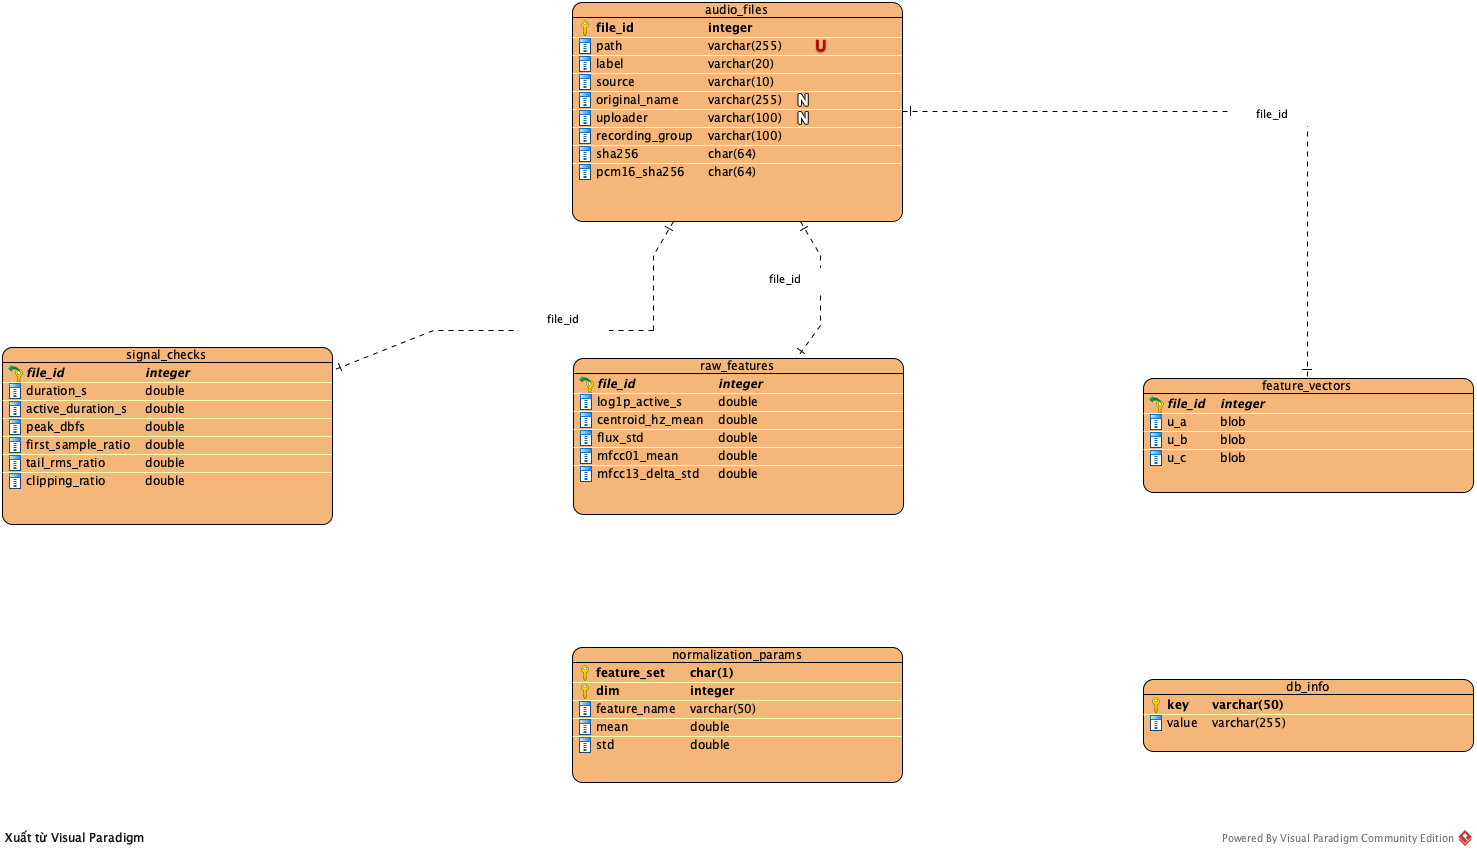
\includegraphics[width=\textwidth]{III_03_ERD_LuocDoCSDL.png}
\caption{Lược đồ cơ sở dữ liệu.}\label{fig:luocdo}
\end{figure}
\begin{table}[htbp]
\centering\small
\caption{Các bảng trong cơ sở dữ liệu.}\label{tab:bang}
\begin{tabularx}{\textwidth}{p{.23\textwidth}rX}
\toprule
Bảng & Số dòng & Nội dung\\\midrule
\texttt{audio\_files} & 655 & Bảng danh mục (Mục~\ref{sec:dinhdang}): mã tệp, đường dẫn, nhãn, nguồn, tên gốc, người tải lên, nhóm bản thu, SHA-256 của tệp và của chuỗi mẫu PCM 16-bit.\\
\texttt{signal\_checks} & 655 & Sáu số đo ở Bảng~\ref{tab:kiemtra}.\\
\texttt{raw\_features} & 655 & Giá trị gốc của 21 thuộc tính A và 39 thuộc tính B, kiểu \texttt{DOUBLE PRECISION}, cột đặt theo tên thuộc tính và thứ tự ở Phụ lục.\\
\texttt{normalization\_params} & 60 & $\mu_j$, $s_j$ của 60 thuộc tính, tính một lần trên 655 tệp (Mục~\ref{sec:chuanhoa}).\\
\texttt{feature\_vectors} & 655 & $u_A$, $u_B$, $u_C$ lưu sẵn để tìm kiếm.\\
\texttt{db\_info} & 6 & Phiên bản dữ liệu, thời điểm tạo, số tệp, số lớp, số chiều, phiên bản thư viện.\\\bottomrule
\end{tabularx}
\end{table}

Cơ sở dữ liệu lưu cả giá trị gốc lẫn vector đã chuẩn hóa. Giá trị gốc là dữ liệu chuẩn: khi đổi cách chuẩn hóa hay trọng số của C thì chỉ cần tính lại \texttt{feature\_vectors}, không phải trích đặc trưng lại từ tệp âm thanh; còn \texttt{feature\_vectors} có sẵn để câu lệnh SQL so sánh trực tiếp trên cột vector. Nhãn nhạc cụ chỉ nằm trong \texttt{audio\_files}, không có trong các bảng đặc trưng, nên phép tìm kiếm chỉ dựa vào âm thanh; nhãn dùng để hiển thị và đánh giá.

\subsection{Ràng buộc toàn vẹn và chỉ mục}
\begin{itemize}
\item \textbf{Khóa:} \texttt{file\_id} là khóa chính của bốn bảng theo tệp; ba bảng phụ tham chiếu \texttt{audio\_files} bằng khóa ngoại. \texttt{path} là duy nhất. Khóa chính của \texttt{normalization\_params} là cặp (\texttt{feature\_set}, \texttt{dim}).
\item \textbf{Ràng buộc \texttt{CHECK}:} các cột của \texttt{signal\_checks} đặt đúng các ngưỡng ở Bảng~\ref{tab:kiemtra}, nên hệ quản trị không nhận tệp không đạt điều kiện chất lượng; ngoài ra $s_j>0$, \texttt{source} và \texttt{feature\_set} chỉ nhận các giá trị hợp lệ.
\item \textbf{Chỉ mục:} B-tree trên \texttt{label} và \texttt{pcm16\_sha256} (nhận ra truy vấn trùng tệp bằng một phép tra cứu); HNSW trên \texttt{u\_a}, \texttt{u\_b}, \texttt{u\_c} theo khoảng cách Euclid (Mục~\ref{sec:cachtim}).
\end{itemize}

\subsection{Ví dụ dữ liệu của một tệp}
Xét tệp kick mã 217 (Freesound, tên gốc ``Kick Fx - Marker \#183.wav''). Trong \texttt{signal\_checks}, tệp dài 0,451 s, đỉnh $-1{,}90$ dBFS, mẫu đầu bằng 4,9\% đỉnh và không có mẫu bị cắt đỉnh. Bảng~\ref{tab:vidu217} theo dõi năm thuộc tính của tệp qua ba bảng đặc trưng.
\begin{table}[htbp]
\centering\small
\caption{Dữ liệu đặc trưng của tệp 217.}\label{tab:vidu217}
\begin{tabular}{llrrrrr}
\toprule
Chiều & Thuộc tính & $x$ & $\mu$ & $s$ & $z$ & $u_C$\\\midrule
A1 & Thời gian có tín hiệu (log) & 0,372 & 0,476 & 0,459 & $-0{,}226$ & $-0{,}0349$\\
A6 & TB trọng tâm phổ (Hz) & 65,8 & 1530,6 & 1698,3 & $-0{,}862$ & $-0{,}1331$\\
A18 & TB tỷ lệ năng lượng dưới 500 Hz & 1,000 & 0,535 & 0,416 & 1,117 & 0,1723\\
B1 & TB MFCC 1 & 29,86 & 9,66 & 12,78 & 1,580 & 0,1789\\
B27 & ĐLC delta MFCC 1 & 0,728 & 0,651 & 0,362 & 0,214 & 0,0242\\\bottomrule
\end{tabular}
\end{table}
Thuộc tính bộ A có $u_C=z/\sqrt{42}$, bộ B có $u_C=z/\sqrt{78}$. Chẳng hạn ở A6, $z=(65{,}8-1530{,}6)/1698{,}3=-0{,}862$ và $u_C=-0{,}862/\sqrt{42}=-0{,}1331$, đúng giá trị lưu trong cột \texttt{u\_c}. Trọng tâm phổ 65,8 Hz và gần 100\% năng lượng dưới 500 Hz là đặc điểm điển hình của kick (Bảng~\ref{tab:acoustic}).

\section{Xây dựng và truy vấn cơ sở dữ liệu}\label{sec:xaydung}
\subsection{Quy trình xây dựng}\label{sec:quytrinhxd}
\begin{enumerate}
\item \textbf{Đọc danh sách tệp} từ bảng kiểm kê và bảng danh mục nguồn; dừng nếu tập tệp WAV thực có khác hai bảng này.
\item \textbf{Gán nhóm bản thu}, gom các tệp có thể đến từ cùng một buổi thu: cùng người tải lên (Freesound), cùng bộ trống (IDMT), cùng nhạc cụ, cách đánh và độ to (Iowa). Kết quả có 136 nhóm, dùng khi đánh giá ở Mục~\ref{sec:danhgia}.
\item \textbf{Trích đặc trưng từng tệp} bằng bước 1--5 ở Mục~\ref{sec:buocxuly}.
\item \textbf{Tính tham số chuẩn hóa} $\mu_j$, $s_j$ trên 655 tệp, rồi tính $u_A$, $u_B$, $u_C$ cho từng tệp.
\item \textbf{Ghi vào cơ sở dữ liệu} trong một giao dịch: tạo lại sáu bảng, ghi dữ liệu và tạo chỉ mục. Lỗi ở bất kỳ bước nào làm giao dịch bị hủy, cơ sở dữ liệu giữ nguyên trạng thái cũ.
\end{enumerate}
Toàn bộ quá trình mất khoảng 2--3 giây; cơ sở dữ liệu chiếm khoảng 11 MB.

\Needspace{12\baselineskip}
\subsection{Truy vấn đặc trưng}
Câu lệnh tìm 5 tệp gần nhất theo bộ C, loại các tệp trùng truy vấn (\texttt{:q} là vector $u_C$ của truy vấn, \texttt{:excluded} là danh sách mã tệp trùng):
\begin{verbatim}
SELECT t.file_id, t.label, v.u_c <-> :q AS d
FROM feature_vectors v JOIN audio_files t USING (file_id)
WHERE v.file_id <> ALL(:excluded) ORDER BY v.u_c <-> :q LIMIT 5;
\end{verbatim}
Danh sách \texttt{:excluded} lấy từ câu \texttt{SELECT file\_id FROM audio\_files WHERE pcm16\_sha256 = :pcm\_hash}.

pgvector lưu mỗi thành phần vector bằng số thực 32 bit, lệch dưới $10^{-6}$ so với giá trị 64 bit mà Bảng~\ref{tab:thietlap} quy định. Vì vậy PostgreSQL chỉ chọn ra 10 ứng viên theo cột vector; chương trình tính lại khoảng cách của 10 ứng viên này bằng số thực 64 bit từ \texttt{raw\_features} và \texttt{normalization\_params} rồi lấy 5 tệp đầu, tệp nào cách đều truy vấn thì tệp có mã nhỏ hơn đứng trước. Kết quả trùng với phép tính 64 bit trên toàn kho (Mục~\ref{sec:dungdan}).
\clearpage

\phan{Tìm kiếm âm thanh tương đồng}
\section{Sơ đồ khối và quy trình}\label{sec:sodokhoi}
\subsection{Sơ đồ khối}
Hệ thống gồm hai luồng (Hình~\ref{fig:sodokhoi}). Luồng xây dựng chạy một lần để đưa 655 tệp vào cơ sở dữ liệu (Phần III). Luồng truy vấn chạy với mỗi tệp âm thanh mới; hai luồng dùng chung các khối M2, M3, M4 và tham số chuẩn hóa $\mu_j, s_j$ lưu trong cơ sở dữ liệu.
\begin{figure}[htbp]
\centering
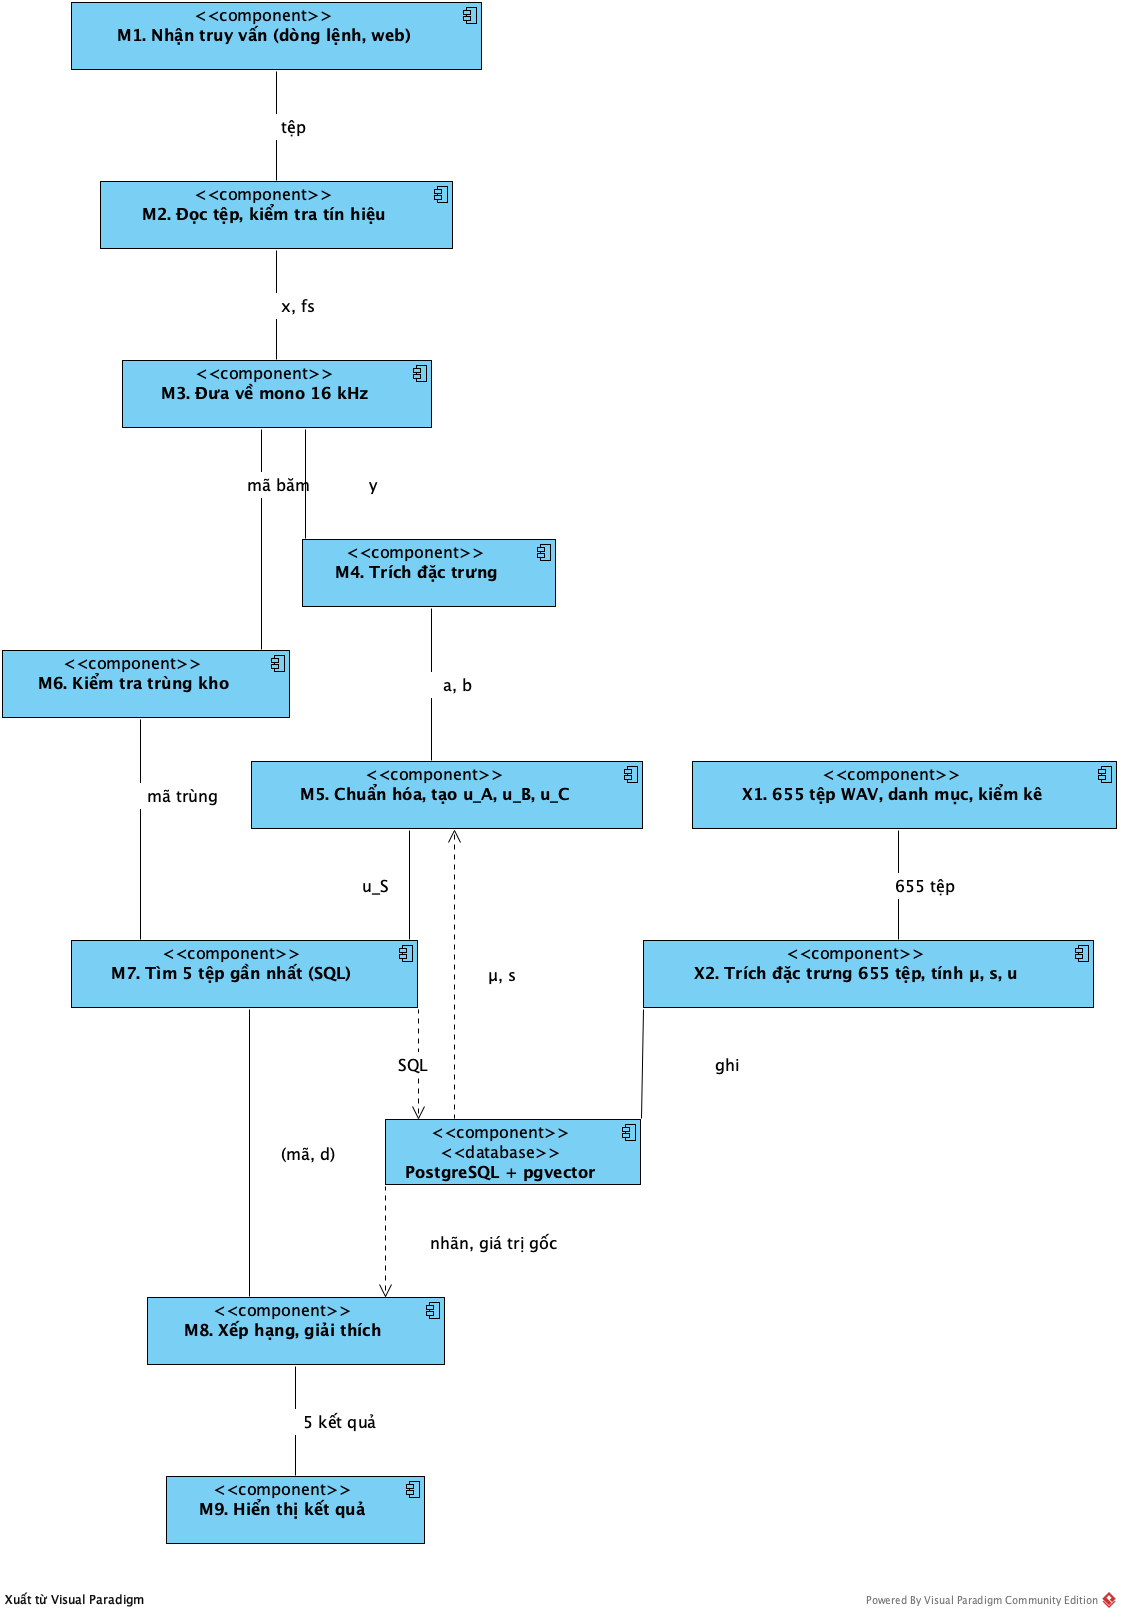
\includegraphics[height=.62\textheight]{IV_04_COMP_SoDoKhoi.png}
\caption{Sơ đồ khối của hệ thống.}\label{fig:sodokhoi}
\end{figure}

\subsection{Chức năng và dữ liệu vào, ra của từng khối}
Bảng~\ref{tab:khoi} mô tả chức năng, dữ liệu vào và dữ liệu ra của từng khối trong Hình~\ref{fig:sodokhoi}. Các khối M2--M5 cài đặt đúng các bước 1--7 của Mục~\ref{sec:quytrinh}; khối M7 là bước 8.
\begin{table}[htbp]
\centering\footnotesize
\caption{Chức năng và dữ liệu vào, ra của các khối.}\label{tab:khoi}
\begin{tabularx}{\textwidth}{>{\raggedright}p{.15\textwidth}>{\raggedright}X>{\raggedright}p{.22\textwidth}>{\raggedright\arraybackslash}p{.22\textwidth}}
\toprule
Khối & Chức năng & Đầu vào & Đầu ra\\\midrule
M1. Nhận truy vấn & Nhận tệp từ dòng lệnh hoặc trang web; chọn bộ đặc trưng (mặc định C) & Tệp WAV, MP3, FLAC, OGG, AIFF\ldots; bộ $S$ & Đường dẫn tệp, $S$\\
M2. Đọc và kiểm tra & Đọc mẫu số thực 64 bit; đo sáu đại lượng ở Bảng~\ref{tab:kiemtra} & Tệp âm thanh & Ma trận mẫu $x$ (mẫu $\times$ kênh), $f_s$, sáu số đo; hoặc thông báo từ chối\\
M3. Chuẩn hóa định dạng & Trộn kênh bằng trung bình; lấy mẫu lại về 16 kHz; tính SHA-256 của PCM 16-bit & $x$, $f_s$ & Tín hiệu mono $y$; mã băm PCM\\
M4. Trích đặc trưng & Bước 2--6 của Mục~\ref{sec:quytrinh} với thiết lập ở Bảng~\ref{tab:thietlap} & $y$ & $a\in\mathbb R^{21}$, $b\in\mathbb R^{39}$\\
M5. Chuẩn hóa & Bước 7: $z_j=(x_j-\mu_j)/s_j$ với $\mu_j, s_j$ đọc từ cơ sở dữ liệu; tạo $u_A,u_B,u_C$ & $a$, $b$, $\mu$, $s$ & $z\in\mathbb R^{60}$; $u_S$\\
M6. Kiểm tra trùng & Tìm tệp trong kho có cùng mã băm PCM & Mã băm & Danh sách mã tệp cần loại\\
M7. Tìm kiếm & Bước 8: câu lệnh SQL \texttt{ORDER BY u <-> q LIMIT 10}; tính lại $d_S$ bằng số thực 64 bit, lấy 5 tệp & $u_S$, mã cần loại & 5 cặp (mã tệp, $d_S$) tăng dần\\
M8. Xếp hạng & Tính $s=1/(1+d)$; lấy nhãn, đường dẫn; tính $d_A,d_B,d_C$ và các thuộc tính A giống, khác nhất theo $|\Delta z|$ & 5 cặp (mã, $d$); danh mục tệp và giá trị đặc trưng gốc & 5 kết quả xếp theo độ tương đồng giảm dần\\
M9. Hiển thị & In ra màn hình, xuất JSON hoặc hiển thị trên web kèm trình phát âm thanh & 5 kết quả, số liệu trung gian & Kết quả cho người dùng\\\midrule
X1, X2. Xây dựng & Chạy M2--M4 cho 655 tệp; tính $\mu,s,u$; ghi vào cơ sở dữ liệu & 655 tệp, bảng danh mục và kiểm kê & Sáu bảng ở Bảng~\ref{tab:bang}\\\bottomrule
\end{tabularx}
\end{table}

\subsection{Quy trình thực hiện một truy vấn}
\begin{enumerate}
\item Người dùng đưa vào một tệp âm thanh và chọn bộ đặc trưng (mặc định C).
\item M2 kiểm tra tín hiệu. Tệp không đạt điều kiện Mục~\ref{sec:curation} bị từ chối và quá trình dừng.
\item M3 đưa tín hiệu về mono 16 kHz; M6 dùng mã băm PCM để nhận ra truy vấn trùng một tệp trong kho.
\item M4 tính 21 giá trị A và 39 giá trị B; M5 chuẩn hóa bằng $\mu_j, s_j$ đã lưu, không tính lại trên truy vấn.
\item M7 gửi câu lệnh SQL đến PostgreSQL, nhận 10 ứng viên, tính lại khoảng cách và giữ 5 tệp gần nhất, đã loại tệp trùng.
\item M8 tính độ tương đồng $s=1/(1+d)$, xếp giảm dần và kèm phần giải thích; M9 trả kết quả.
\end{enumerate}
Với nhạc cụ chưa có trong kho, quy trình vẫn như trên và hệ thống trả 5 tệp có đặc trưng gần nhất. Hình~\ref{fig:hoatdong} là sơ đồ hoạt động của quy trình này.
\begin{figure}[htbp]
\centering
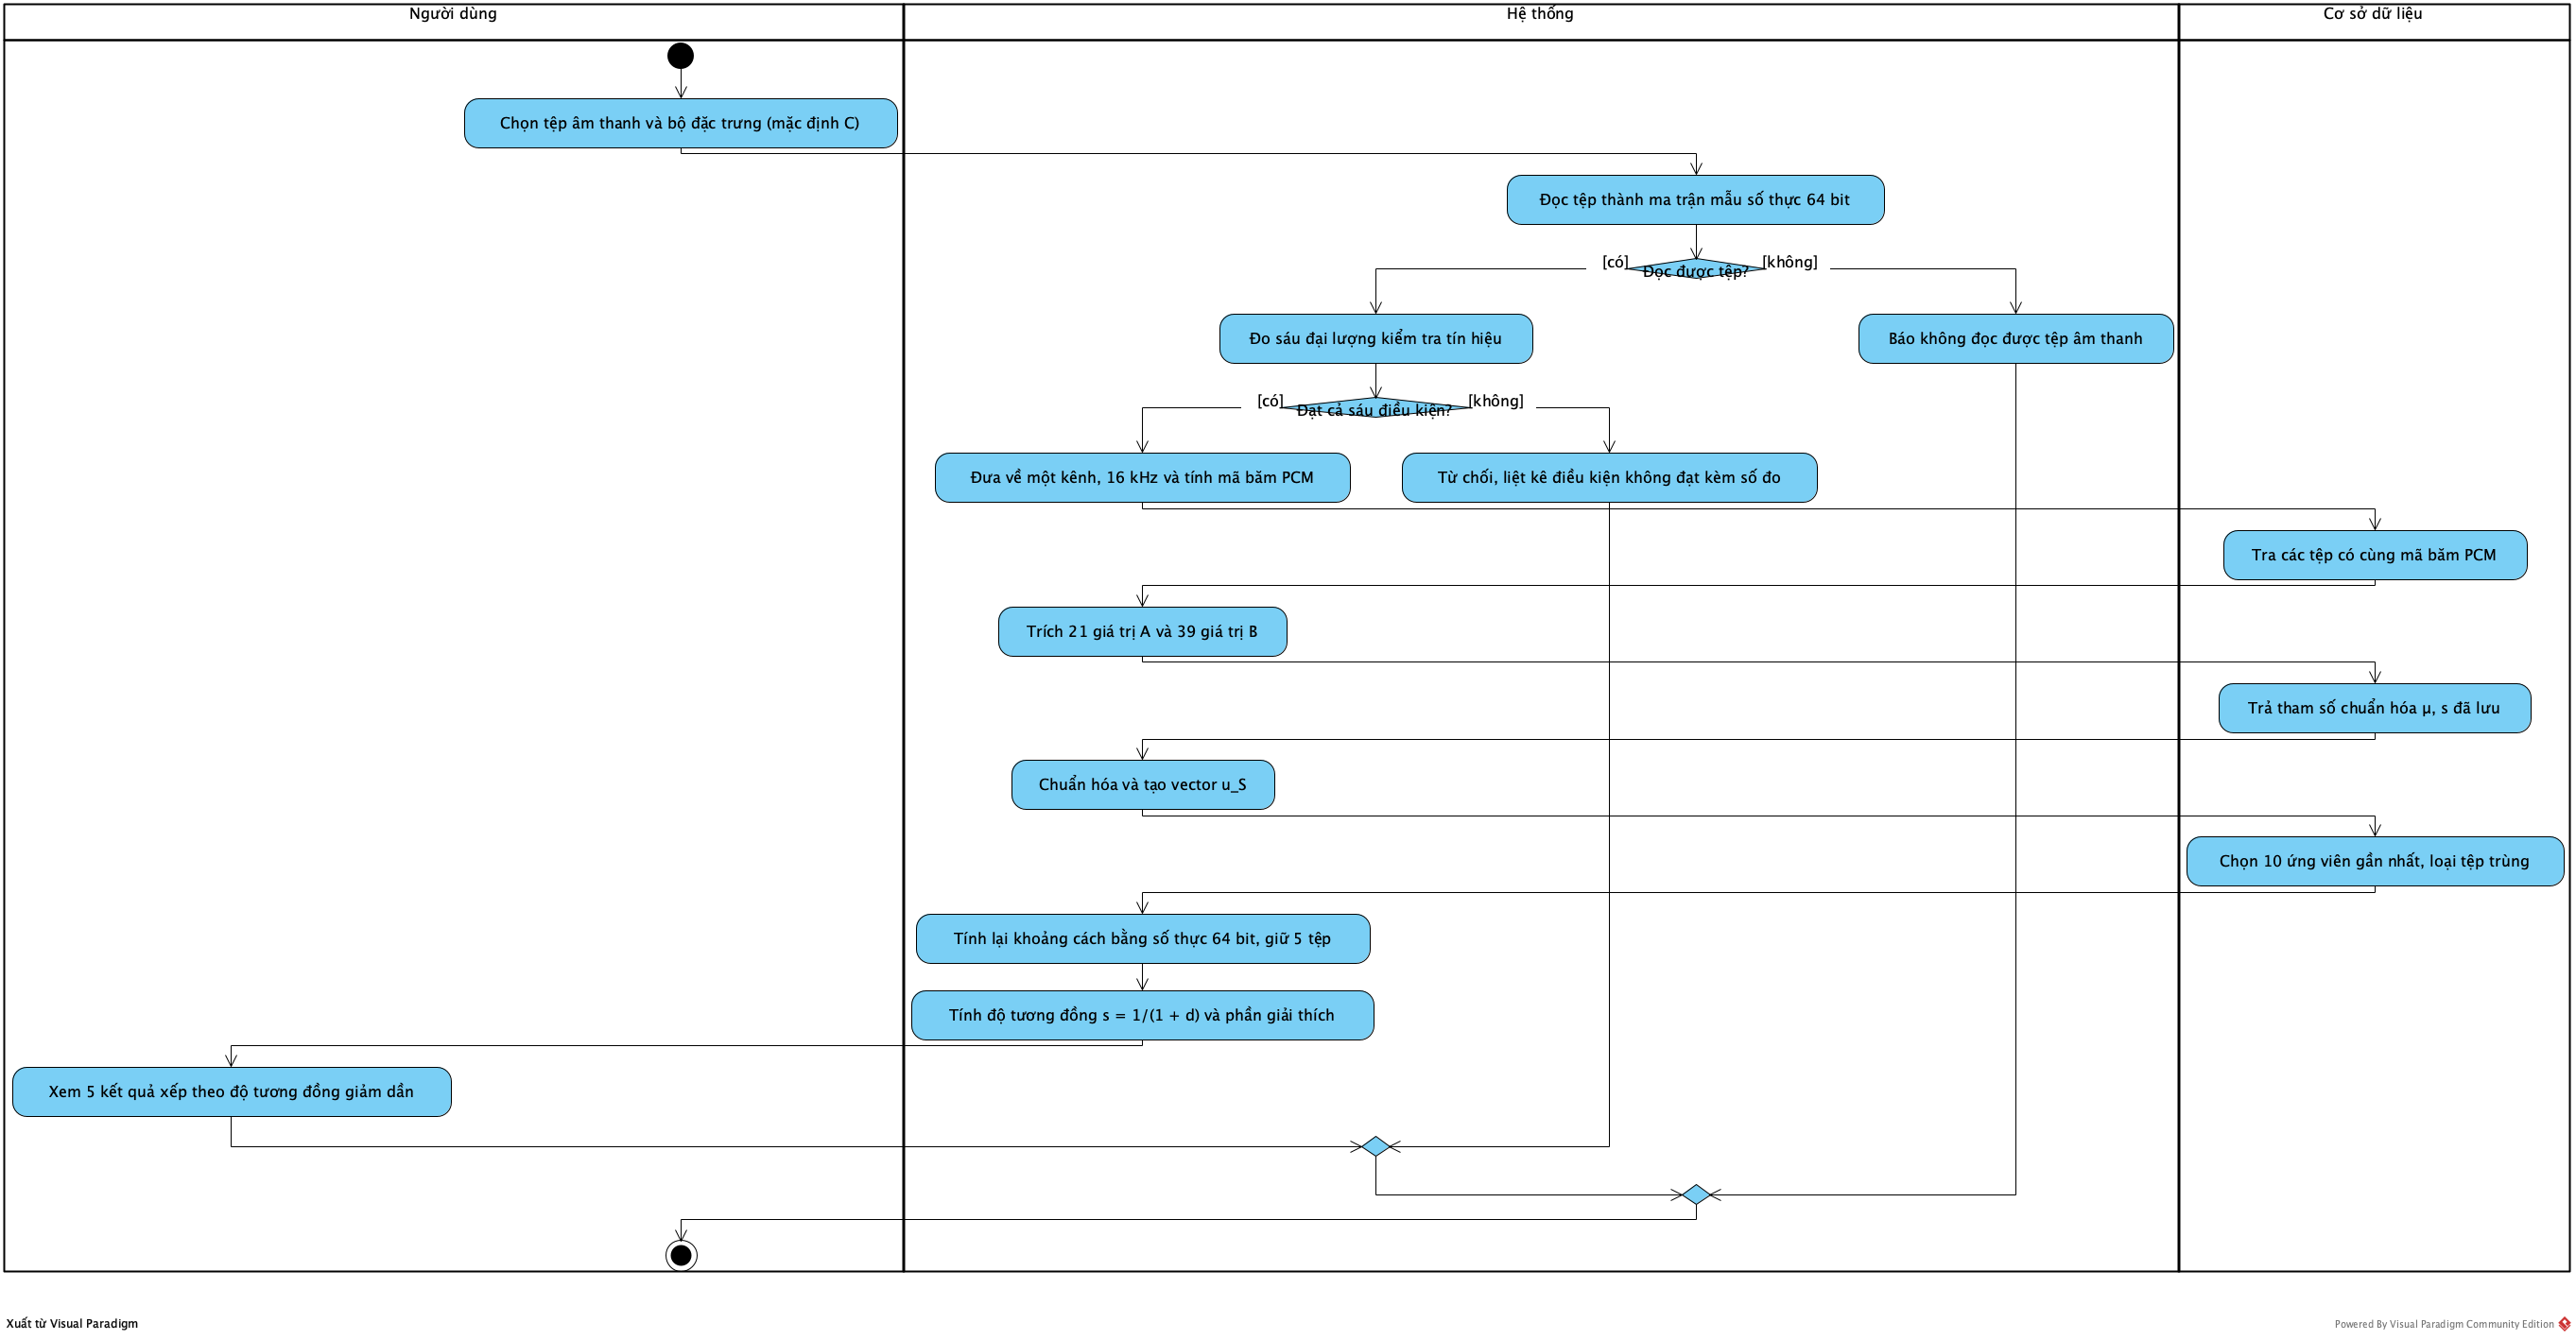
\includegraphics[width=\textwidth]{IV_05_ACT_XuLyTruyVan.png}
\caption{Sơ đồ hoạt động xử lý truy vấn.}\label{fig:hoatdong}
\end{figure}

\subsection{Cách tìm 5 tệp gần nhất}\label{sec:cachtim}
Bước 8 có thể thực hiện theo ba cách cho cùng một kết quả:
\begin{itemize}
\item \textbf{pgvector} (mặc định): PostgreSQL thực hiện câu lệnh SQL ở Mục~\ref{sec:xaydung}.
\item \textbf{Cây k-d}: chương trình dựng một cây k-d trong bộ nhớ cho mỗi bộ đặc trưng. Ở mỗi nút, chiều chia là chiều có độ trải lớn nhất trong nhánh, điểm chia là trung vị theo chiều đó. Khi tìm, nhánh bên kia chỉ được xét nếu khoảng cách từ truy vấn đến siêu phẳng chia nhỏ hơn khoảng cách đến láng giềng thứ 5 đang giữ.
\item \textbf{Vét cạn}: tính khoảng cách đến mọi tệp rồi sắp xếp; dùng để kiểm chứng hai cách trên.
\end{itemize}
Bảng~\ref{tab:cachtim} so sánh các cách trên 655 truy vấn bỏ-một-ra. Cây k-d bỏ qua được khoảng một nửa số tệp ở bộ A (21 chiều), nhưng ở B và C vẫn phải tính khoảng cách tới khoảng 98\% số tệp. Đây là hiện tượng đã biết của các cấu trúc phân hoạch không gian khi số chiều lớn: các điểm có khoảng cách xấp xỉ nhau nên hầu hết các nhánh đều không bị loại.

Chỉ mục HNSW là phương pháp tìm \emph{xấp xỉ}. Khi bắt buộc dùng chỉ mục, 5 kết quả trùng với kết quả vét cạn ở 99,85--100\% các vị trí. Với 655 dòng, bộ tối ưu truy vấn của PostgreSQL tự chọn quét tuần tự vì rẻ hơn dùng chỉ mục, nên kết quả mặc định vẫn chính xác.
\begin{table}[htbp]
\centering\small
\caption{So sánh ba cách tìm 5 tệp gần nhất.}\label{tab:cachtim}
\begin{tabular}{lrrrr}
\toprule
Bộ & Số chiều & Cây k-d: số tệp phải tính TB & Tỷ lệ so với 654 & HNSW bắt buộc: trùng vét cạn\\\midrule
A & 21 & 357,6 & 54,7\% & 100,00\%\\
B & 39 & 640,5 & 97,9\% & 99,91\%\\
C & 60 & 640,8 & 98,0\% & 99,85\%\\\bottomrule
\end{tabular}
\end{table}
Hệ thống chọn pgvector làm cách mặc định vì phép tìm được thực hiện ngay trong hệ quản trị cơ sở dữ liệu, kết quả chính xác và có sẵn chỉ mục khi kho mở rộng. Cây k-d và vét cạn dùng để đối chiếu.

\section{Minh họa kết quả trung gian}\label{sec:minhhoa}
Mục này minh họa ba truy vấn với các tệp nằm ngoài kho, lấy từ tập Freesound One-Shot Percussive Sounds: một nhạc cụ đã có lớp trong kho, một nhạc cụ chưa có và một tệp bị từ chối. Nhãn của các tệp này lấy theo thông tin mô tả của nguồn. Các số liệu dưới đây đều dùng bộ C (mặc định).

\subsection{Truy vấn nhạc cụ đã có: một tiếng kick mới}
Tệp truy vấn là một tiếng kick (mã Freesound 185294), dài 0,395 s. Mã băm PCM không trùng tệp nào trong kho.

Ở bước kiểm tra tín hiệu, thời gian có tiếng 0,170 s, đỉnh $-1{,}92$ dBFS, mẫu đầu bằng 0,6\% đỉnh và RMS khối cuối bằng 0,2\% đỉnh. Không có mẫu nào chạm $|x|\ge0{,}999$. Tệp đạt cả sáu điều kiện ở Bảng~\ref{tab:kiemtra}.

Ở bước trích đặc trưng và chuẩn hóa, Bảng~\ref{tab:vd_dactrung} trích 8 trong 60 thuộc tính: giá trị gốc $x$, tham số $\mu, s$ đọc từ cơ sở dữ liệu, giá trị chuẩn hóa $z$ và thành phần tương ứng của $u_C$ ($z/\sqrt{42}$ với A, $z/\sqrt{78}$ với B). Tệp có trọng tâm phổ 72 Hz và 99,9\% năng lượng dưới 500 Hz, đúng đặc điểm của kick ở Bảng~\ref{tab:acoustic}. Hình~\ref{fig:hoso} vẽ $z$ của cả 60 chiều.
\begin{table}[htbp]
\centering\small
\caption{Giá trị trung gian của truy vấn kick.}\label{tab:vd_dactrung}
\begin{tabular}{llrrrrrr}
\toprule
& & \multicolumn{4}{c}{Truy vấn} & \multicolumn{2}{c}{Kết quả hạng 1}\\
\cmidrule(lr){3-6}\cmidrule(lr){7-8}
Chiều & Thuộc tính & $x$ & $\mu$ & $s$ & $z$ & $z$ & $(\Delta u)^2$\\\midrule
A1 & Thời gian có tín hiệu (log) & 0,157 & 0,476 & 0,459 & $-0{,}695$ & $-0{,}658$ & 0,00003\\
A3 & Hệ số đỉnh (dB) & 12,442 & 15,712 & 3,820 & $-0{,}856$ & $-0{,}333$ & 0,00652\\
A6 & TB trọng tâm phổ (Hz) & 72,2 & 1.530,6 & 1.698,3 & $-0{,}859$ & $-0{,}837$ & 0,00001\\
A12 & TB độ phẳng phổ & 0,000002 & 0,0844 & 0,1230 & $-0{,}686$ & $-0{,}683$ & 0,00000\\
A18 & TB tỷ lệ năng lượng dưới 500 Hz & 0,9993 & 0,5348 & 0,4164 & 1,116 & 1,112 & 0,00000\\
A20 & TB thông lượng phổ & 0,282 & 0,238 & 0,132 & 0,334 & 0,624 & 0,00199\\
B1 & TB MFCC 1 & 37,026 & 9,663 & 12,781 & 2,141 & 1,004 & 0,01657\\
B2 & TB MFCC 2 & 7,652 & 2,563 & 7,077 & 0,719 & 0,592 & 0,00021\\\bottomrule
\end{tabular}
\end{table}
\begin{figure}[htbp]
\centering
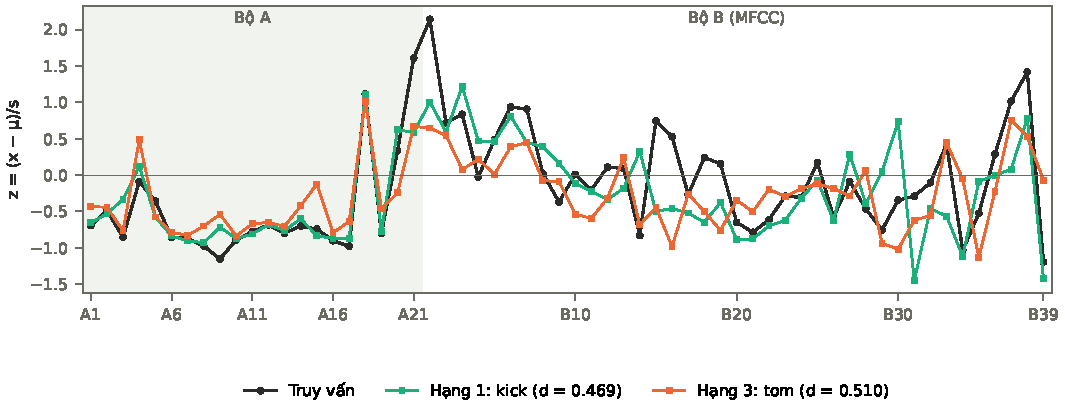
\includegraphics[width=\textwidth]{hinh4_ho_so_z.pdf}
\caption{Giá trị chuẩn hóa $z$ của truy vấn kick và hai kết quả.}\label{fig:hoso}
\end{figure}

Ở bước tìm kiếm, sau khi PostgreSQL trả về các ứng viên, chương trình tính lại khoảng cách và giữ 5 tệp gần nhất (Bảng~\ref{tab:vd_ketqua}).
\begin{table}[htbp]
\centering\small
\caption{Kết quả truy vấn kick.}\label{tab:vd_ketqua}
\begin{tabular}{rrllrrrr}
\toprule
Hạng & Mã tệp & Nguồn & Nhãn & $d_A$ & $d_B$ & $d_C$ & $s=1/(1+d_C)$\\\midrule
1 & 248 & Freesound 35656 & kick & 0,2875 & 0,5971 & 0,4686 & 0,6809\\
2 & 256 & Freesound 88627 & kick & 0,3123 & 0,6397 & 0,5034 & 0,6652\\
3 & 573 & Freesound 33169 & tom & 0,3702 & 0,6189 & 0,5099 & 0,6623\\
4 & 332 & Freesound 35650 & kick & 0,2396 & 0,7125 & 0,5315 & 0,6529\\
5 & 270 & Freesound 35664 & kick & 0,3604 & 0,6770 & 0,5423 & 0,6484\\\bottomrule
\end{tabular}
\end{table}

Độ tương đồng của kết quả hạng 1 được tính như sau. Cộng $(\Delta u)^2$ trên 21 chiều A được $0{,}04133=\tfrac12d_A^2$, trên 39 chiều B được $0{,}17829=\tfrac12d_B^2$. Do đó
\[
d_C=\sqrt{\tfrac12\cdot0{,}2875^2+\tfrac12\cdot0{,}5971^2}=\sqrt{0{,}04133+0{,}17829}=0{,}4686,\qquad s=\frac{1}{1+0{,}4686}=0{,}6809.
\]
Chiều đóng góp nhiều nhất vào $d_C^2$ là ĐLC thông lượng phổ (A21, 0,0250), tiếp theo là ĐLC MFCC 2 (B15, 0,0198). Phần giải thích của hệ thống so sánh $|\Delta z|$ trên bộ A: hai tệp gần như trùng nhau ở tỷ lệ năng lượng dưới 500 Hz, độ phẳng phổ và tần số cắt ($|\Delta z|<0{,}02$), và khác nhau nhiều nhất ở ĐLC thông lượng phổ ($1{,}03\sigma$) và hệ số đỉnh ($0{,}52\sigma$).

Bốn trong năm kết quả là kick; kết quả hạng 3 là tom, có $d_A$ và $d_B$ đều gần kết quả hạng 2. Kết quả này khớp với nhận xét ở Mục~\ref{sec:cap}: kick và tom cùng là trống màng rung có năng lượng dồn ở dải thấp. Hình~\ref{fig:vd_pho} cho thấy cả năm kết quả đều có khởi âm ngắn và năng lượng tập trung dưới 1 kHz như truy vấn.
\begin{figure}[htbp]
\centering
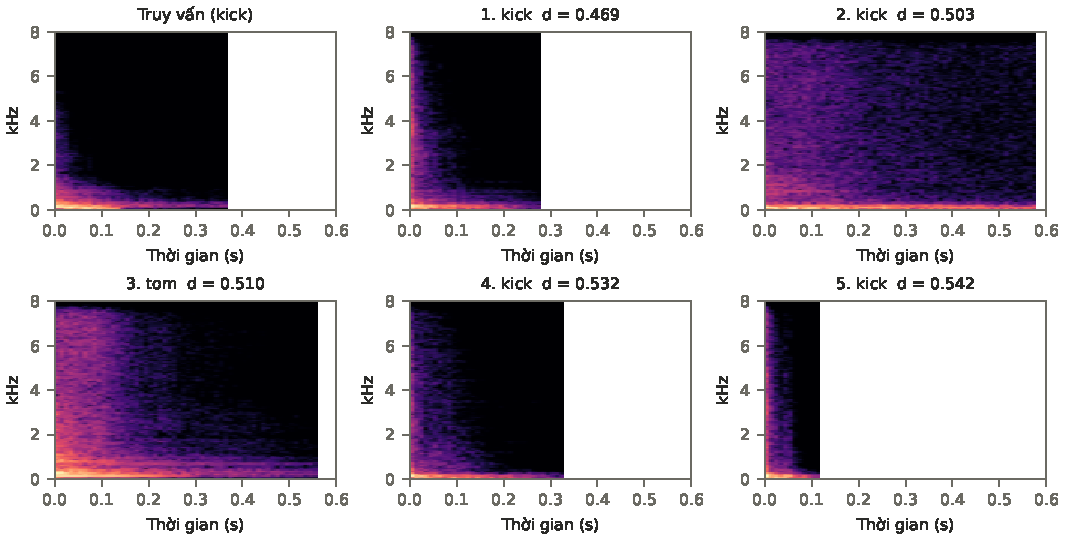
\includegraphics[width=\textwidth]{hinh3_vi_du_truy_van.pdf}
\caption{Phổ đồ truy vấn kick và 5 kết quả.}\label{fig:vd_pho}
\end{figure}

\subsection{Truy vấn nhạc cụ chưa có trong kho: djembe}
Djembe là trống màng rung không thuộc 13 lớp của kho. Tệp truy vấn (mã Freesound 54015) dài 0,255 s, đạt cả sáu điều kiện kiểm tra tín hiệu. Hệ thống trả về bốn tom và một conga, đều là trống màng rung (Bảng~\ref{tab:vd_ngoai}, Hình~\ref{fig:vd_ngoai}).
\begin{table}[htbp]
\centering\small
\caption{Kết quả truy vấn djembe.}\label{tab:vd_ngoai}
\begin{tabular}{rrllrrrr}
\toprule
Hạng & Mã tệp & Nguồn & Nhãn & $d_A$ & $d_B$ & $d_C$ & $s$\\\midrule
1 & 583 & Freesound 193508 & tom & 0,4524 & 1,0096 & 0,7823 & 0,5611\\
2 & 630 & Freesound 33174 & tom & 0,4938 & 1,0509 & 0,8210 & 0,5491\\
3 & 45 & Freesound 455509 & conga & 0,4293 & 1,0838 & 0,8243 & 0,5482\\
4 & 619 & Freesound 16318 & tom & 0,4183 & 1,0988 & 0,8313 & 0,5460\\
5 & 566 & Freesound 171235 & tom & 0,4814 & 1,0846 & 0,8391 & 0,5437\\\bottomrule
\end{tabular}
\end{table}
\begin{figure}[htbp]
\centering
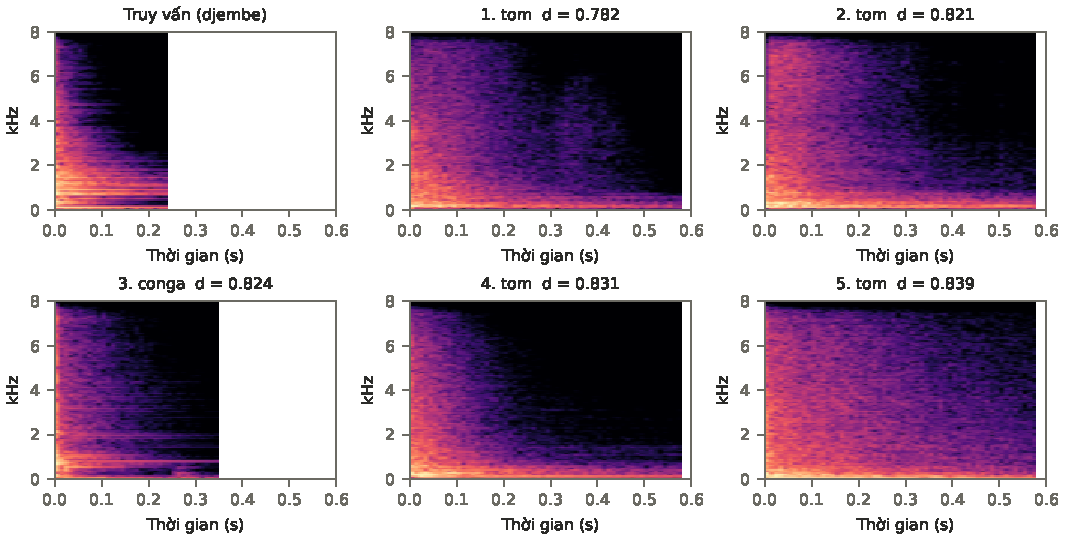
\includegraphics[width=\textwidth]{hinh6_vi_du_ngoai_kho.pdf}
\caption{Phổ đồ truy vấn djembe và 5 kết quả.}\label{fig:vd_ngoai}
\end{figure}
Khoảng cách $d_C$ của các kết quả (0,78--0,84) lớn hơn hẳn so với truy vấn kick (0,47--0,54), chủ yếu do $d_B$: hình dạng bao phổ của djembe khác các trống trong kho. Độ tương đồng vì vậy thấp hơn (0,54--0,56). Phần giải thích cho thấy kết quả hạng 1 gần truy vấn về độ phẳng phổ và tần số cắt, nhưng khác ở tỷ lệ năng lượng dưới 500 Hz ($1{,}05\sigma$): djembe có 48,6\% năng lượng dưới 500 Hz, so với khoảng 92\% của tom này.

\subsection{Truy vấn bị từ chối và truy vấn trùng kho}
Một tiếng maracas (mã Freesound 9697) chỉ dài 0,036 s, phần có tiếng 0,030 s. Hệ thống từ chối với thông báo: ``Không đạt điều kiện chất lượng (Mục 2): dài 0,036 s $<$ 0,1 s; phần có tiếng 0,030 s $<$ 0,05 s''. Khi truy vấn là một tệp trong kho, khối M6 tìm được mã tệp có cùng mã băm PCM và loại tệp đó; 5 kết quả là 5 tệp khác gần nhất.

\section{Đánh giá kết quả}\label{sec:danhgia}
\subsection{Phương pháp đánh giá}
Đề bài yêu cầu sắp xếp theo độ tương đồng nội dung, nhưng bộ dữ liệu không có nhãn đánh giá tương đồng do người nghe gán. Vì vậy nhóm dùng \emph{nhãn nhạc cụ} làm tiêu chí gián tiếp: một kết quả được coi là phù hợp khi cùng nhãn với truy vấn. Các chỉ số gồm:
\begin{itemize}
\item \textbf{P@5:} tỷ lệ kết quả cùng nhãn trong 5 kết quả;
\item \textbf{Hạng 1 đúng:} kết quả đầu tiên cùng nhãn;
\item \textbf{Bỏ phiếu:} nhãn xuất hiện nhiều nhất trong 5 kết quả trùng nhãn truy vấn.
\end{itemize}
Mỗi chỉ số được tính theo hai cách: trung bình trên mọi truy vấn (TV) và trung bình đều trên 13 lớp (Lớp), để lớp nhỏ không bị kick, snare lấn át.

Các phép đánh giá được thực hiện trên kho 655 tệp:
\begin{enumerate}
\item \textbf{Bỏ-một-ra:} lần lượt dùng từng tệp làm truy vấn, tìm trong 654 tệp còn lại.
\item \textbf{Chia theo nhóm bản thu:} 136 nhóm bản thu được chia vào 5 phần, mỗi phần 131 tệp. Tệp của một phần làm truy vấn, tìm trong 4 phần còn lại; $\mu_j, s_j$ chỉ tính trên 4 phần đó. Truy vấn và kho không bao giờ cùng nhóm bản thu. 16 truy vấn agogo bị bỏ vì cả lớp nằm trong một nhóm, nên còn 639 truy vấn.
\item \textbf{Độ bền:} truy vấn là bản biến đổi của từng tệp trong kho; kiểm tra bản gốc có được tìm lại hay không.
\item \textbf{Nhạc cụ ngoài kho:} mô tả nhãn của các kết quả khi truy vấn là nhạc cụ chưa có.
\item \textbf{Tính đúng đắn và thời gian.}
\end{enumerate}

\subsection{Kết quả theo bộ đặc trưng}
\begin{table}[htbp]
\centering\small
\caption{Kết quả tìm kiếm của ba bộ đặc trưng.}\label{tab:ketqua}
\begin{tabular}{llrrrrrr}
\toprule
& & \multicolumn{2}{c}{P@5} & \multicolumn{2}{c}{Hạng 1 đúng} & \multicolumn{2}{c}{Bỏ phiếu}\\
\cmidrule(lr){3-4}\cmidrule(lr){5-6}\cmidrule(lr){7-8}
Đánh giá & Bộ & TV & Lớp & TV & Lớp & TV & Lớp\\\midrule
Bỏ-một-ra & A & 0,799 & 0,674 & 0,863 & 0,805 & 0,843 & 0,717\\
(655 truy vấn) & B & 0,730 & 0,622 & 0,815 & 0,766 & 0,795 & 0,670\\
& C & \textbf{0,832} & \textbf{0,741} & \textbf{0,896} & \textbf{0,869} & \textbf{0,866} & \textbf{0,778}\\\midrule
Theo nhóm bản thu & A & 0,621 & 0,446 & 0,684 & 0,562 & 0,656 & 0,441\\
(639 truy vấn) & B & 0,571 & 0,424 & 0,649 & 0,560 & 0,610 & 0,461\\
& C & \textbf{0,666} & \textbf{0,521} & \textbf{0,728} & \textbf{0,654} & \textbf{0,695} & \textbf{0,535}\\\bottomrule
\end{tabular}
\end{table}
Bộ C đạt cao nhất ở mọi chỉ số của cả hai cách đánh giá (Bảng~\ref{tab:ketqua}). Ghép MFCC vào A làm $Q$ giảm (Bảng~\ref{tab:Q}) nhưng làm P@5 tăng. $Q$ đo khoảng cách trung bình trên toàn bộ các cặp tệp, còn tìm kiếm chỉ xét 5 láng giềng gần nhất. Thông tin bao phổ của B giúp phân biệt các tệp ở gần nhau, dù trung bình toàn cục kém tách hơn.

Các chỉ số khi chia theo nhóm bản thu thấp hơn cách bỏ-một-ra khoảng 0,17 điểm P@5. Trong bỏ-một-ra, kho thường còn các tệp khác của cùng người tải lên hoặc cùng bộ trống với truy vấn; khi tách theo nhóm, hệ thống phải tìm tệp cùng nhạc cụ từ nguồn thu khác, nên chỉ số này phản ánh sát hơn trường hợp truy vấn là một bản thu mới.

\begin{figure}[htbp]
\centering
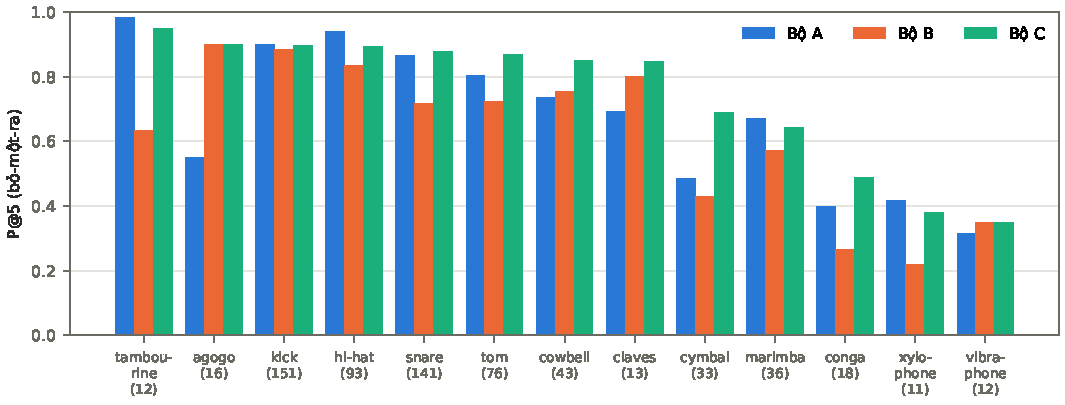
\includegraphics[width=\textwidth]{hinh5_p5_theo_lop.pdf}
\caption{P@5 theo từng lớp.}\label{fig:p5lop}
\end{figure}
Hình~\ref{fig:p5lop} cho thấy tambourine, agogo, kick, hi-hat, snare đạt P@5 từ 0,88 trở lên với bộ C. Các lớp thấp nhất trùng với những cặp gần nhau đã nêu ở Phần I:
\begin{itemize}
\item conga (0,49): 41 trong 90 vị trí kết quả là tom; conga/tom có khoảng cách tâm nhỏ nhất ở Bảng~\ref{tab:cap};
\item vibraphone (0,35): 36 trong 60 vị trí là marimba; marimba (0,64) nhầm chủ yếu sang kick và vibraphone, do năng lượng tập trung ở dải thấp (Bảng~\ref{tab:acoustic});
\item xylophone (0,38): nhầm sang cowbell, kick, snare; lớp chỉ có 11 tệp;
\item cymbal (0,69): nhầm sang snare, cùng nhóm phổ phân tán.
\end{itemize}
Theo nguồn, P@5 của bộ C là 0,917 với IDMT, 0,841 với Freesound và 0,571 với Iowa; các lớp của Iowa (marimba, vibraphone) chịu ảnh hưởng của nốt được chơi như đã nêu ở Mục~\ref{sec:cap}.

\subsection{Lựa chọn bộ đặc trưng mặc định}\label{sec:chonbo}
Mục~\ref{sec:sudung} chọn A làm bộ mặc định ban đầu dựa trên $Q$ và để kết quả tìm kiếm quyết định bộ cuối cùng. Theo Bảng~\ref{tab:ketqua}, C có P@5, tỷ lệ hạng 1 đúng và tỷ lệ bỏ phiếu đúng cao nhất ở cả bỏ-một-ra lẫn chia theo nhóm bản thu, tính theo truy vấn và theo lớp, nên hệ thống dùng bộ C làm mặc định; A và B vẫn chọn được khi truy vấn. B nhạy với nén MP3 (Mục~\ref{sec:doben}), nên với truy vấn MP3 bộ A tìm lại bản gốc tốt hơn C.

\subsection{Độ bền với biến đổi tín hiệu}\label{sec:doben}
Mỗi tệp trong kho được biến đổi rồi dùng làm truy vấn; bản gốc vẫn ở trong kho. Bảng~\ref{tab:doben} cho tỷ lệ bản gốc xuất hiện ở hạng 1 và P@5 tính trên 5 kết quả còn lại sau khi bỏ bản gốc.
\begin{table}[htbp]
\centering\small
\caption{Độ bền với biến đổi tín hiệu.}\label{tab:doben}
\begin{tabular}{lrrrrrrr}
\toprule
& & \multicolumn{3}{c}{Bản gốc ở hạng 1} & \multicolumn{3}{c}{P@5 không tính bản gốc}\\
\cmidrule(lr){3-5}\cmidrule(lr){6-8}
Biến đổi & Số truy vấn & A & B & C & A & B & C\\\midrule
Stereo, 44,1 kHz & 655 & 0,994 & 0,998 & 0,997 & 0,795 & 0,729 & 0,832\\
Giảm âm lượng 20 dB & 624 & 0,997 & 0,973 & 0,990 & 0,802 & 0,736 & 0,840\\
Nén MP3, 44,1 kHz & 655 & 0,973 & 0,792 & 0,849 & 0,794 & 0,697 & 0,809\\
Thêm nhiễu trắng, SNR 30 dB & 654 & 0,528 & 0,581 & 0,642 & 0,601 & 0,623 & 0,683\\\bottomrule
\end{tabular}
\end{table}
\begin{itemize}
\item \textbf{Stereo 44,1 kHz:} sau khi đưa về mono 16 kHz, bản gốc gần như luôn ở hạng 1.
\item \textbf{Giảm âm lượng:} đặc trưng không phụ thuộc độ to nhờ chuẩn hóa đỉnh (Mục~\ref{sec:quytrinh}). 31 truy vấn bị từ chối vì tệp gốc có đỉnh dưới $-20$ dBFS, nên sau khi giảm 20 dB thì dưới ngưỡng $-40$ dBFS của Mục~\ref{sec:curation}.
\item \textbf{Nén MP3:} bộ A ít bị ảnh hưởng; MFCC (B) nhạy với phần phổ bị bộ mã hóa thay đổi.
\item \textbf{Nhiễu trắng:} ảnh hưởng mạnh nhất, vì nhiễu làm tăng độ phẳng phổ, ZCR và năng lượng ở các đoạn im lặng, đúng những thuộc tính có $J_j$ cao ở Bảng~\ref{tab:J}. Một truy vấn bị từ chối vì mẫu đầu vượt 10\% đỉnh.
\end{itemize}

\subsection{Truy vấn bằng nhạc cụ ngoài kho}\label{sec:ngoaikho}
Nhóm dùng 73 tệp thuộc 12 loại nhạc cụ không có trong kho, lấy từ cùng tập Freesound. Nhãn của các tệp lấy theo thông tin mô tả của nguồn nên chỉ mang tính tham khảo. 4 tệp (một cabasa, hai maracas, một shaker) bị từ chối vì dài dưới 0,1 s, còn 69 tệp đều nhận đủ 5 kết quả. Không có đáp án ``đúng'' cho các truy vấn này, nên Bảng~\ref{tab:ngoaikho} chỉ mô tả kết quả: nhãn thường gặp nhất và tỷ lệ kết quả cùng họ nhạc cụ theo Bảng~\ref{tab:phanloai}, không phải số đo độ chính xác.
\begin{table}[htbp]
\centering\small
\caption{Kết quả với nhạc cụ ngoài kho.}\label{tab:ngoaikho}
\begin{tabularx}{\textwidth}{lrlXrrr}
\toprule
& & & & \multicolumn{3}{c}{Cùng họ}\\\cmidrule(lr){5-7}
Nhạc cụ & Số tệp & Họ & Nhãn kết quả thường gặp (bộ C) & A & B & C\\\midrule
djembe & 24 & màng rung & tom 60, kick 41, cowbell 9, conga 5 & 0,76 & 0,85 & 0,92\\
bongo & 7 & màng rung & conga 11, snare 11, tom 10 & 0,71 & 0,71 & 0,97\\
tabla & 1 & màng rung & tom 3, kick 2 & 1,00 & 1,00 & 1,00\\
gong & 8 & kim loại & cowbell 15, snare 8, tom 7, cymbal 5 & 0,47 & 0,68 & 0,50\\
triangle & 2 & kim loại & cymbal 5, hi-hat 4, tambourine 1 & 0,70 & 0,80 & 1,00\\
castanets & 15 & gỗ & snare 44, claves 20, cymbal 10 & 0,13 & 0,08 & 0,27\\
woodblock & 4 & gỗ & snare 8, kick 4, tom 3, cowbell 2 & 0,25 & 0,00 & 0,05\\
cajon & 3 & gỗ & tom 8, kick 5 & 0,00 & 0,00 & 0,00\\
maracas, shaker, vibraslap & 5 & -- & hi-hat 9, snare 9, cymbal 5, tambourine 2 & -- & -- & --\\\bottomrule
\end{tabularx}
\end{table}
Các trống màng rung (djembe, bongo, tabla) được ghép với tom, conga, kick; triangle được ghép với cymbal và hi-hat. Các nhạc cụ gỗ ít khi nhận kết quả cùng họ vì họ này trong kho chỉ có claves (13 tệp). Castanets vẫn nhận claves ở 20 trong 75 vị trí. Cajon là hộp gỗ nhưng được chơi như trống trầm, nên kết quả là tom và kick; các nhạc cụ lắc nhận các lớp phổ phân tán như hi-hat, snare.

\subsection{Tính đúng đắn và thời gian xử lý}\label{sec:dungdan}
\begin{itemize}
\item Ba cách tìm (pgvector, cây k-d, vét cạn) cho kết quả trùng nhau ở 655/655 truy vấn bỏ-một-ra của cả ba bộ, cả thứ tự lẫn khoảng cách.
\item 17 phép kiểm thử tự động đều đạt. Các phép kiểm thử gồm: cây k-d trùng vét cạn khi có điểm trùng nhau; vector trong PostgreSQL khớp giá trị 64 bit; truy vấn trùng kho bị loại; bản stereo 44,1 kHz tìm lại bản gốc; tệp im lặng, hỏng, quá nhỏ, mất khởi âm, cắt đuôi hoặc cắt đỉnh bị từ chối; ràng buộc \texttt{CHECK} hoạt động; giao diện web xử lý đúng tệp tải lên và yêu cầu sai.
\end{itemize}
Trên máy tính của nhóm, trung vị thời gian trên 100 truy vấn là khoảng 1 ms cho đọc tệp, kiểm tra và trích đặc trưng. Phần tìm 5 tệp gần nhất với bộ C mất khoảng 1--2 ms qua PostgreSQL, 1,2 ms với cây k-d và 0,1 ms với vét cạn bằng NumPy. Thời gian qua PostgreSQL chủ yếu là chi phí gửi nhận câu lệnh.

\subsection{Nhận xét chung}
\enlargethispage{2\baselineskip}
Hệ thống nhận tệp mới ở nhiều định dạng và trả đúng 5 tệp xếp theo độ tương đồng giảm dần, kể cả với nhạc cụ chưa có trong kho. Với bộ C, trung bình 4,2/5 kết quả cùng nhạc cụ với truy vấn (bỏ-một-ra) và 3,3/5 khi truy vấn khác nhóm bản thu. Kết quả kém nhất ở các cặp lớp gần nhau (conga/tom, marimba/vibraphone) và các lớp ít tệp. P@5 dựa trên nhãn nhạc cụ, chưa phải đánh giá của người nghe.
\clearpage

\section*{Kết luận}
\phantomsection\addcontentsline{toc}{part}{Kết luận}
Nhóm đã thực hiện Yêu cầu 1--4 của đề tài:
\begin{enumerate}
\item Bộ dữ liệu 655 tệp WAV thuộc 13 lớp nhạc cụ bộ gõ từ ba nguồn, kèm mô tả đặc điểm giống và khác nhau giữa các lớp (Phần I).
\item Ba bộ đặc trưng A (21 chiều), B (39 chiều) và C (60 chiều), với công thức, ý nghĩa và giá trị thông tin của từng thuộc tính (Phần II).
\item Công cụ trích rút đặc trưng dùng chung một mã nguồn cho kho và truy vấn. Hệ cơ sở dữ liệu PostgreSQL + pgvector gồm sáu bảng, có ràng buộc theo đúng các điều kiện chất lượng; giá trị lưu trữ trùng bảng đặc trưng của Phần II (Phần III).
\item Hệ thống tìm 5 tệp tương đồng nhất cho tệp âm thanh mới, kể cả nhạc cụ chưa có trong kho. Hệ thống được mô tả bằng sơ đồ khối, minh họa các giá trị trung gian và được đánh giá bằng nhiều phép thử. Bộ C đạt P@5 bằng 0,832 khi bỏ-một-ra và 0,666 khi tách theo nhóm bản thu, cao nhất trong ba bộ, nên được chọn làm mặc định (Phần IV).
\end{enumerate}
Cơ sở dữ liệu và các kết quả đánh giá đều có thể tạo lại từ mã nguồn kèm theo.
\clearpage

\section*{Phụ lục: danh sách thuộc tính của các bộ đặc trưng}
\phantomsection\addcontentsline{toc}{part}{Phụ lục: danh sách thuộc tính của các bộ đặc trưng}
Bảng~\ref{tab:thuoctinh} liệt kê thứ tự các chiều dùng trong vector và trong cơ sở dữ liệu. ``TB'' và ``ĐLC'' lần lượt là trung bình và độ lệch chuẩn trên khung hợp lệ. Trong A, mỗi cặp thuộc tính theo khung được xếp TB trước, ĐLC sau. Cách ghép và trọng số của C được quy định ở Mục~\ref{sec:boC}.
\begin{table}[htbp]
\centering\small
\caption{Thuộc tính của bộ A và bộ B.}\label{tab:thuoctinh}
\begin{tabularx}{\textwidth}{clccX}
\toprule
Chiều & Thuộc tính & Ký hiệu & Đơn vị & Định nghĩa\\\midrule
\multicolumn{5}{l}{\textbf{Bộ A: 5 thuộc tính thời gian}}\\
A1 & Thời gian có tín hiệu (log) & $a_1$ & -- & $\ln(1+T_a)$, Mục~\ref{sec:boA-tg}\\
A2 & Khoảng chứa 90\% năng lượng (log) & $a_2$ & -- & $\ln(1+D_{90})$\\
A3 & Hệ số đỉnh & $a_3$ & dB & Đỉnh so với RMS vùng có tín hiệu\\
A4 & Tỷ lệ có tín hiệu & $a_4$ & -- & $T_a/T_s$\\
A5 & Vị trí đỉnh bao RMS & $a_5$ & -- & Vị trí tương đối trong vùng có tín hiệu\\\midrule
\multicolumn{5}{l}{\textbf{Bộ A: 16 thuộc tính phổ (TB và ĐLC của 8 đại lượng)}}\\
A6--A7 & Trọng tâm phổ & $C$ & Hz & Mục~\ref{sec:boA-pho}\\
A8--A9 & Độ rộng phổ & $W$ & Hz & \\
A10--A11 & Tần số cắt 85\% & $R$ & Hz & \\
A12--A13 & Độ phẳng phổ & $F$ & -- & \\
A14--A15 & Entropy phổ & $H$ & -- & \\
A16--A17 & Tỷ lệ đổi dấu & $Z$ & -- & \\
A18--A19 & Tỷ lệ năng lượng dưới 500 Hz & $L$ & -- & \\
A20--A21 & Thông lượng phổ dương & $\Phi$ & -- & \\\midrule
\multicolumn{5}{l}{\textbf{Bộ B: 39 thuộc tính MFCC}}\\
B1--B13 & TB của MFCC 1 đến 13 & $c[1..13]$ & -- & Mục~\ref{sec:boB}\\
B14--B26 & ĐLC của MFCC 1 đến 13 & $c[1..13]$ & -- & \\
B27--B39 & ĐLC của delta MFCC 1 đến 13 & $\Delta c[1..13]$ & -- & \\\bottomrule
\end{tabularx}
\end{table}
\clearpage

\begin{thebibliography}{99}
\phantomsection\addcontentsline{toc}{part}{Tài liệu tham khảo}
\bibitem{freesound} A. Ramires, P. Chandna, X. Favory, E. Gómez và X. Serra. \emph{Freesound One-Shot Percussive Sounds}, Version 1.0, Zenodo. DOI: 10.5281/zenodo.4687854. \url{https://zenodo.org/records/4687854}.
\bibitem{idmt} Fraunhofer IDMT. \emph{IDMT-SMT-Drums}. \url{https://www.idmt.fraunhofer.de/en/publications/datasets/drums.html}. Gói dữ liệu: \url{https://zenodo.org/records/7544164}.
\bibitem{iowa} L. Fritts, University of Iowa Electronic Music Studios. \emph{Musical Instrument Samples}. \url{https://theremin.music.uiowa.edu/MIS.html}.
\bibitem{mfcc} S. B. Davis và P. Mermelstein. Comparison of parametric representations for monosyllabic word recognition in continuously spoken sentences. \emph{IEEE Transactions on Acoustics, Speech, and Signal Processing}, 28(4):357--366, 1980.
\bibitem{peeters} G. Peeters. \emph{A large set of audio features for sound description (similarity and classification) in the CUIDADO project}. Báo cáo kỹ thuật, IRCAM, 2004.
\bibitem{dct} SciPy Developers. \emph{scipy.fft.dct}. \url{https://docs.scipy.org/doc/scipy/reference/generated/scipy.fft.dct.html}. Phiên bản SciPy dùng khi tính dữ liệu: 1.17.1.
\bibitem{postgres} PostgreSQL Global Development Group. \emph{PostgreSQL 17 Documentation}. \url{https://www.postgresql.org/docs/17/}.
\bibitem{pgvector} A. Kane và cộng sự. \emph{pgvector: Open-source vector similarity search for Postgres}, phiên bản 0.8.0. \url{https://github.com/pgvector/pgvector}.
\bibitem{hnsw} Y. A. Malkov và D. A. Yashunin. Efficient and robust approximate nearest neighbor search using Hierarchical Navigable Small World graphs. \emph{IEEE Transactions on Pattern Analysis and Machine Intelligence}, 42(4):824--836, 2020.
\bibitem{kdtree} J. L. Bentley. Multidimensional binary search trees used for associative searching. \emph{Communications of the ACM}, 18(9):509--517, 1975.
\bibitem{friedman} J. H. Friedman, J. L. Bentley và R. A. Finkel. An algorithm for finding best matches in logarithmic expected time. \emph{ACM Transactions on Mathematical Software}, 3(3):209--226, 1977.
\bibitem{weber} R. Weber, H.-J. Schek và S. Blott. A quantitative analysis and performance study for similarity-search methods in high-dimensional spaces. \emph{Proceedings of the 24th VLDB Conference}, 194--205, 1998.
\bibitem{manning} C. D. Manning, P. Raghavan và H. Schütze. \emph{Introduction to Information Retrieval}, chương 8. Cambridge University Press, 2008.
\end{thebibliography}
\end{document}
